\documentclass[a4paper,titlepage]{article}

\makeatletter
\def\input@path{{../../../template/}{./img}}
\makeatother

\usepackage{Comandi}
\usepackage{Riferimenti}
\usepackage{Stile}

\usepackage{eurosym}
\usepackage{comment}
\usepackage{hyperref}

% -- COMANDI PER LE COMPONENTI -- %
\newenvironment{componente}[1]
{
	\subsubsection{Componente \texttt{#1}}
	\label{#1}
	Informazioni sul package
	\begin{itemize}
}{
	\end{itemize}
}
\newcommand{\compDescrizione}[1] {
	\item \textbf{Descrizione}: {#1}
}
\newcommand{\compPadre}[1] {
	\item \textbf{Padre}: {#1}
}
\newcommand{\compUtilizzo}[1] {
	\item \textbf{Utilizzo}: {#1}
}
\newenvironment{compPackageContenuti}[1] {
	\item \textbf{Package contenuti}: {#1}
	\begin{itemize}
} {
	\end{itemize}
}
\newenvironment{compClassi} [1] {
	\item \textbf{Classi}: {#1}
	\begin{itemize}
} {
	\end{itemize}
}
\newenvironment{classe} [1] {
	\item[] \texttt{#1} \\
	\begin{itemize}
} {
	\end{itemize}
}
\newcommand{\classeDescrizione} [1] { \\
	\item \textbf{Descrizione}: {#1}
}
\newcommand{\classeUtilizzo} [1] { \\
	\item \textbf{Utilizzo}: {#1}
}
\newenvironment{classeAttributi} [1] { \\
	\item \textbf{Attributi}: {#1}
	\begin{itemize}
} {
	\end{itemize}
}
\newcommand{\classeAttributo}[3] { \item \texttt{{#1}: {#2}} {#3}}
\newenvironment{classeMetodi} [1] {
	\item \textbf{Metodi}: {#1}
	\begin{itemize}
} {
	\end{itemize}
}
\newcommand{\classeMetodo}[4]{
	\item \texttt{{#1}}%({#2}) : {#3}} \\ {#4}
}
\newenvironment{classeMetodoArgomenti} {
	\item \textbf{Argomenti}:
	\begin{itemize}
}{
	\end{itemize}
}
\newcommand{\classeMetodoArgomento}[3]{\item \texttt{{#1} : {#2}} \\ {#3} }
\newenvironment{classeRelazioni} { \\
	\item \textbf{Relazioni con altre classi}:
	\begin{itemize}
} {
	\end{itemize}
}
\newcommand{\classeRelazione}[3]{\item \textt{#1::#2}: {#3}}


\def\NOME{Specifica Tecnica}
\def\VERSIONE{1.0.0}
\def\DATA{2016-06-10}
\def\REDATTORE{Viviana Alessio \\ & Matteo Franco \\ & Andrea Grandene \\ & Luca Soldera}
\def\VERIFICATORE{Enrico Bellio \\ & Tommaso Panozzo}
\def\RESPONSABILE{Matteo Franco}
\def\USO{Esterno}
\def\DESTINATARI{\COMMITTENTE \\ & \CARDIN \\ & \PROPONENTE}
\def\SOMMARIO{Descrizione dell'architettura ad alto livello per il \gl{progetto} \PROGETTO.}

\begin{document}


\maketitle

\begin{diario}

	\modifica{Matteo Franco}{\RES}{Approvazione documento}{2016-06-10}{1.0.0}

		\modifica{Viviana Alessio}{\PRJ}{Correzione errori classi}{2016-06-09}{0.2.0}
		\modifica{Tommaso Panozzo}{\VER}{Verifica classi inserite}{2016-06-09}{0.1.9}

	\modifica{Andrea Grendene}{\PRJ}{Inserimento classi package server}{2016-06-07}{0.1.9}
	\modifica{Andrea Grendene}{\PRJ}{Inserimento classi package server--urlrequesthandler}{2016-06-07}{0.1.9}
	\modifica{Andrea Grendene}{\PRJ}{Inserimento classi package server--data}{2016-06-07}{0.1.9}

		\modifica{Viviana Alessio}{\PRJ}{Correzione errori ortografici e sintattici}{2016-06-05}{0.1.9}
		\modifica{Enrico Bellio}{\VER}{Verifica classi inserite}{2016-06-05}{0.1.8}

	\modifica{Luca Soldera}{\PRJ}{Inserimento classi package client--data}{2016-06-04}{0.1.8}
	\modifica{Luca Soldera}{\PRJ}{Inserimento classi package client--datamanager}{2016-06-04}{0.1.8}
	\modifica{Luca Soldera}{\PRJ}{Inserimento classi package client--location}{2016-06-04}{0.1.8}
	\modifica{Luca Soldera}{\PRJ}{Inserimento classi package client--pathprogress}{2016-06-04}{0.1.8}
	\modifica{Luca Soldera}{\PRJ}{Inserimento classi package client--urlrequest}{2016-06-04}{0.1.8}
	\modifica{Luca Soldera}{\PRJ}{Inserimento classi package client}{2016-06-04}{0.1.8}

		\modifica{Viviana Alessio}{\PRJ}{Correzione errori classi}{2016-06-04}{0.1.8}
		\modifica{Enrico Bellio}{\VER}{Verifica classi inserite}{2016-06-04}{0.1.7}

	\modifica{Matteo Franco}{\PRJ}{Inserimento classi package client--viewcontroller}{2016-05-30}{0.1.7}
	\modifica{Matteo Franco}{\PRJ}{Inserimento classi package client--viewcontroller--utility}{2016-05-30}{0.1.7}
	\modifica{Matteo Franco}{\PRJ}{Inserimento classi package client--viewcontroller--savedresults}{2016-05-30}{0.1.7}
	\modifica{Matteo Franco}{\PRJ}{Inserimento classi package client--viewcontroller--games}{2016-05-30}{0.1.7}
	\modifica{Matteo Franco}{\PRJ}{Inserimento classi package client--viewcontroller--building}{2016-05-30}{0.1.7}
	\modifica{Matteo Franco}{\PRJ}{Inserimento classi package client--viewcontroller--authentication}{2016-05-30}{0.1.7}

	\modifica{Viviana Alessio}{\PRJ}{Correzione errori ortografici e sintattici}{2016-05-28}{0.1.7}
	\modifica{Tommaso Panozzo}{\VER}{Verifica packages inseriti}{2016-05-27}{0.1.6}

	\modifica{Andrea Grendene}{\PRJ}{Inserimento package server}{2016-05-26}{0.1.6}
	\modifica{Andrea Grendene}{\PRJ}{Inserimento package server--urlrequesthandler}{2016-05-26}{0.1.6}
	\modifica{Andrea Grendene}{\PRJ}{Inserimento package server--data}{2016-05-26}{0.1.6}
	\modifica{Luca Soldera}{\PRJ}{Inserimento package client--data}{2016-05-26}{0.1.6}
	\modifica{Luca Soldera}{\PRJ}{Inserimento package client--datamanager}{2016-05-26}{0.1.5}
	\modifica{Luca Soldera}{\PRJ}{Inserimento package client--location}{2016-05-26}{0.1.5}
	\modifica{Luca Soldera}{\PRJ}{Inserimento package client--pathprogress}{2016-05-26}{0.1.5}
	\modifica{Luca Soldera}{\PRJ}{Inserimento package client--urlrequest}{2016-05-26}{0.1.5}
	\modifica{Luca Soldera}{\PRJ}{Inserimento package client}{2016-05-26}{0.1.5}
	\modifica{Matteo Franco}{\PRJ}{Inserimento package client--viewcontroller}{2016-05-26}{0.1.5}
	\modifica{Matteo Franco}{\PRJ}{Inserimento package client--viewcontroller--utility}{2016-05-26}{0.1.5}
	\modifica{Matteo Franco}{\PRJ}{Inserimento package client--viewcontroller--savedresults}{2016-05-26}{0.1.4}
	\modifica{Matteo Franco}{\PRJ}{Inserimento package client--viewcontroller--games}{2016-05-26}{0.1.4}
	\modifica{Matteo Franco}{\PRJ}{Inserimento package client--viewcontroller--building}{2016-05-26}{0.1.4}
	\modifica{Matteo Franco}{\PRJ}{Inserimento package client--viewcontroller--authentication}{2016-05-26}{0.1.4}

	\modifica{Viviana Alessio}{\PRJ}{Correzione errori ortografici e sintattici}{2016-05-25}{0.1.4}
	\modifica{Tommaso Panozzo}{\VER}{Verifica sezioni concluse}{2016-05-24}{0.1.3}

	\modifica{Viviana Alessio}{\PRJ}{Stesura sezione \hyperref[architettura]{Descrizione architettura}}{2016-05-23}{0.1.3}
	\modifica{Viviana Alessio}{\PRJ}{Stesura sezione \hyperref[attivita]{Diagrammi delle attività}}{2016-05-22}{0.1.3}
	\modifica{Viviana Alessio}{\PRJ}{Stesura appendice \hyperref[pattern]{Design pattern utilizzati}}{2016-05-21}{0.1.2}
	\modifica{Viviana Alessio}{\PRJ}{Stesura sezione \hyperref[tecnologie]{Tecnologie}}{2016-05-13}{0.1.1}
	\modifica{Viviana Alessio}{\PRJ}{Stesura sezione \hyperref[introduzione]{Introduzione}}{2016-05-12}{0.1.0}
	\modifica{Viviana Alessio}{\PRJ}{Stesura indice}{2016-05-10}{0.0.2}
	\modifica{Matteo Franco}{\PRJ}{Creazione documento}{2016-05-09}{0.0.1}
\end{diario}

\newpage
\tableofcontents
\newpage
\listoftables
\newpage
\listoffigures
\newpage

\section{Introduzione}
	\subsection{Scopo del documento} 
	Questo documento ha lo scopo di spiegare dettagliatamente le strategie secondo cui il gruppo \AUTORE{} intende condurre il \gl{progetto} didattico. 
	\subsection{Scopo del \gl{prodotto}}
	\SCOPO
	\subsection{Glossario}
	\GLOSSARIO
	\subsection{Riferimenti}
		\subsubsection{Normativi}
			\begin{itemize}
				\item \textbf{Capitolato d'appalto C2 - CLIPS:} Communication \& Localisation with Indoor Positioning Systems. \\
				\url{http://www.math.unipd.it/~tullio/IS-1/2015/Progetto/C2.pdf}
				\item \textbf{Vincoli e dettagli tecnico-economici} \\
				\url{http://www.math.unipd.it/~tullio/IS-1/2015/Dispense/PD01.pdf}
				\item \textbf{Norme di Progetto} \\ \NPdoc
				\item \textbf{Regolamento di Progetto} \\
				\url{http://www.math.unipd.it/~tullio/IS-1/2015/Progetto/}
				\item \textbf{Regolamento organigramma} \\
				\url{http://www.math.unipd.it/~tullio/IS-1/2015/Progetto/PD01b.html}
			\end{itemize}	
			
		\subsubsection{Informativi}
			\begin{itemize}
				\item \textbf{Software Engineering (10th edition}) \\
				Ian Sommerville \\
				Pearson Education | Addison-Wesley
				\item \textbf{Guide to the Software Engineering Body of Knowledge}
				IEEE Computer Society. Software Engineering Coordinating Committee
				\item \textbf{Slides del \COMMITTENTE} \\ riguardo i  \href{http://www.math.unipd.it/~tullio/IS-1/2015/Dispense/L02.pdf}{processi \gl{software}}, il \href{http://www.math.unipd.it/~tullio/IS-1/2015/Dispense/L03.pdf}{ciclo di vita del \gl{software}} e \href{http://www.math.unipd.it/~tullio/IS-1/2015/Dispense/L04.pdf}{la gestione di \gl{progetto}}	
			\end{itemize}
	\subsection{Modello di ciclo di vita scelto}
	È stato scelto come ciclo di vita il modello \gl{incrementale}. Le motivazioni che ci hanno spinto verso questa direzione sono il modo in cui è strutturato il \gl{progetto} didattico e la quasi totale inesperienza dei componenti del gruppo nello sviluppare progetti \gl{software} di grandi dimensioni. Di seguito una lista di caratteristiche del metodo \gl{incrementale}:
	\begin{itemize}
		\item si può produrre valore ad ogni incremento;
		\item ogni incremento riduce il rischio di fallimento;
		\item prevede rilasci multipli;
		\item i requisiti utente sono classificati e trattati in base alla loro importanza strategica. I requisiti più importanti sono già stabili all'inizio dello sviluppo del \gl{progetto};
		\item l'analisi dei requisiti e la progettazione architetturale non vengono ripetute;
		\item prima si pensa allo sviluppo dei requisiti essenziali, poi a quelli desiderabili;
		\item Sono presenti delle iterazioni del tipo Prototipo $\rightarrow$ Validazione $\rightarrow$ Prototipo $\rightarrow$ Validazione $\rightarrow$ ecc..
	\end{itemize}
	\subsection{Scadenze}
	Il gruppo Beacon Strips ha deciso di rispettare le seguenti scadenze:
	\begin{itemize} 
		\item \textbf{Revisione dei Requisiti}: 2016-04-18
		\item \textbf{Revisione di Progettazione}: 2016-06-17
		\item \textbf{Revisione di Qualifica}: 2016-08-24
		\item \textbf{Revisione di Accettazione}: 2016-09-12
	\end{itemize}
	In base a queste scadenze e a fronte dell'analisi dei rischi verranno decise le fasi in cui suddividere il lavoro di sviluppo del \gl{progetto}.
	\subsubsection{Scelta Revisione di Progettazione}
	Si è deciso di affrontare la RP$_{\mbox{\textit{min}}}$. Il gruppo si impegna quindi per il 2016-06-17 di presentare nel documento ``Specifica Tecnica'' la progettazione ad alto livello del \gl{prodotto}.
	

\section{Tecnologie utilizzate} 
Per lo sviluppo del progetto abbiamo la necessità di utlizzare delle tecnologie che sono state scelte dopo attenta analisi. 


\section{Descrizione architettura} 
\label{architettura}
	In questa sezione verrà descritta lo schema generale dell'architettura, nella sezione successiva % aggiungere label
	verranno riportate tutti i packages e le classi dettagliatamente.
	 Per i diagrammi delle classi e di attività è stato utilizzato il formalismo UML 2.0. \\
	 L'architettura descritta in questo documento è ad alto livello. Classi, sottoclassi e attributi verranno descritti più dettagliatamente nel periodo in cui attueremo la Progettazione di dettaglio. \\
	 Si procederà nella descrizione dell'architettura con un approccio top-down. Saranno descritte prima quindi le parti più generali per poi andare sempre più nello specifico. Si procederà quindi prima con la descizione dei packages e delle componenti, per poi passare alle singole classi. Successivamente verranno descritti i design pattern utilizzati.
	
	\subsection{Architettura generale}
	L'architettura generale dell'applicazione segue il modello client - server. \\
	In particolare si utilizzerà lo stile architetturale REST (representational state transfer) per coordinare compomenti, connettori e dati attraverso un sistema ipermediale distribuito dove l'attenzione è data al ruolo delle componenti.
	
	\begin{itemize}
		\item \textbf{Vantaggi}: REST offre una interfaccia che separa il client dal server. Questa separazione 
	\end{itemize}
		
		rest - A uniform interface separates clients from servers. This separation of concerns means that, for example, clients are not concerned with data storage, which remains internal to each server, so that the portability of client code is improved. Servers are not concerned with the user interface or user state, so that servers can be simpler and more scalable. Servers and clients may also be replaced and developed independently, as long as the interface between them is not altered.

\begin{componente}{CLIPS}
\compDescrizione{package generale contenente il prodotto del progetto}
\begin{compPackageContenuti}
\item CLIPS::client: componente globale per il front end del prodotto che utilizza il design pattern \gl{MVC}. Si occupa di fornire un'interfaccia grafica dell'applicazione e di interagire con il lato server.
\item CLIPS::server: componente globale per il back end del prodotto
\end{compPackageContenuti}
\end{componente}
\begin{componente}{CLIPS::client}
\compDescrizione{componente globale per il front end del prodotto che utilizza il design pattern \gl{MVC}. Si occupa di fornire un'interfaccia grafica dell'applicazione e di interagire con il lato server.}
\compPadre{CLIPS}
\begin{compPackageContenuti}
\item CLIPS::client::authentication: componente che si occupa di gestire l'autenticazione dell'utente
\item CLIPS::client::data: package per la gestione in locale dei dati
\item CLIPS::client::location: componente che gestisce l'individuazione e la lettura dei beacon
\item CLIPS::client::pathprogress: componente che gestisce i dati del percorso e salva i risultati ottenuti nelle prove mentre si sta giocando
\item CLIPS::client::viewcontroller: componente che raggruppa tutte le view ed i controller relativi alle view
\end{compPackageContenuti}
\end{componente}
\begin{componente}{CLIPS::client::authentication}
\compDescrizione{componente che si occupa di gestire l'autenticazione dell'utente}
\compPadre{client}
\begin{compClassi}
\begin{classe}{CLIPS::client::authentication::AccountActivity}
\classeDescrizione{classe controller che si occupa di interagire con AccountView}
\classeUtilizzo{si occupa di gestire le interazioni dell'utente con AccountView}
\begin{classeRelazioni}
\classeRelazione{CLIPS::client::authentication}{AccountViewDelegate}{interfaccia per segnalare gli eventi della classe AccountView}\end{classeRelazioni}
\end{classe}\begin{classe}{CLIPS::client::authentication::AccountView}
\classeDescrizione{classe che rappresenta la schermata delle informazioni dell'utente}
\classeUtilizzo{permette all'utente di visualizzare le informazioni del proprio profilo}
\begin{classeRelazioni}
\classeRelazione{CLIPS::client::authentication}{AccountActivity}{classe controller che si occupa di interagire con AccountView}\classeRelazione{CLIPS::client::authentication}{AccountViewDelegate}{interfaccia per segnalare gli eventi della classe AccountView}\end{classeRelazioni}
\end{classe}\begin{classe}{CLIPS::client::authentication::AccountViewDelegate}
\classeDescrizione{interfaccia per segnalare gli eventi della classe AccountView}
\classeUtilizzo{si occupa di fornire i metodi necessari alla classe AccountView per notificare gli eventi}
\begin{classeRelazioni}
\classeRelazione{CLIPS::client::authentication}{AccountActivity}{classe controller che si occupa di interagire con AccountView}\classeRelazione{CLIPS::client::authentication}{AccountView}{classe che rappresenta la schermata delle informazioni dell'utente}\end{classeRelazioni}
\end{classe}\begin{classe}{CLIPS::client::authentication::ForgotPasswordActivity}
\classeDescrizione{classe controller che si occupa di interagire con ForgotPasswordView}
\classeUtilizzo{si occupa di gestire le interazioni dell'utente con ForgotPasswordView}
\begin{classeRelazioni}
\classeRelazione{CLIPS::client::authentication}{ForgotPasswordView}{classe che si occupa della visualizzazione della schermata per la richiesta di una nuova password}\classeRelazione{CLIPS::client::authentication}{ForgotPasswordViewDelegate}{interfaccia per segnalare gli eventi della classe ForgotPasswordView}\end{classeRelazioni}
\end{classe}\begin{classe}{CLIPS::client::authentication::ForgotPasswordView}
\classeDescrizione{classe che si occupa della visualizzazione della schermata per la richiesta di una nuova password}
\classeUtilizzo{consente all'utente di inserire la mail per ricevere una nuova password}
\begin{classeAttributi}
\classeAttributo{emailTextField}{TextField}{text field dell'email}
\end{classeAttributi}
\begin{classeRelazioni}
\classeRelazione{CLIPS::client::authentication}{ForgotPasswordViewDelegate}{interfaccia per segnalare gli eventi della classe ForgotPasswordView}\end{classeRelazioni}
\end{classe}\begin{classe}{CLIPS::client::authentication::ForgotPasswordViewDelegate}
\classeDescrizione{interfaccia per segnalare gli eventi della classe ForgotPasswordView}
\classeUtilizzo{si occupa di fornire i metodi necessari alla classe ForgotPasswordView per notificare gli eventi}
\begin{classeRelazioni}
\classeRelazione{CLIPS::client::authentication}{ForgotPasswordActivity}{classe controller che si occupa di interagire con ForgotPasswordView}\classeRelazione{CLIPS::client::authentication}{ForgotPasswordView}{classe che si occupa della visualizzazione della schermata per la richiesta di una nuova password}\end{classeRelazioni}
\end{classe}\begin{classe}{CLIPS::client::authentication::LoginActivity}
\classeDescrizione{classe controller che si occupa di interagire con LoginView}
\classeUtilizzo{si occupa di gestire le interazioni dell'utente con LoginView}
\begin{classeRelazioni}
\classeRelazione{CLIPS::client::authentication}{LoginView}{classe che si occupa della visualizzazione della schermata per il login}\classeRelazione{CLIPS::client::authentication}{LoginViewDelegate}{interfaccia per segnalare gli eventi della classe LoginView}\end{classeRelazioni}
\end{classe}\begin{classe}{CLIPS::client::authentication::LoginView}
\classeDescrizione{classe che si occupa della visualizzazione della schermata per il login}
\classeUtilizzo{consente all'utente di inserire i propri dati per effettuare il login}
\begin{classeAttributi}
\classeAttributo{emailTextField}{string}{rappresenta l'email}
\end{classeAttributi}
\begin{classeMetodi}
\classeMetodo{forgotPasswordPressed()}{}{void}{invia un evento il quale notifica che il bottone di password dimenticata è stato premuto}
\classeMetodo{loginButtonPressed()}{}{void}{invia un evento di bottone del login premuto}
\end{classeMetodi}
\begin{classeRelazioni}
\classeRelazione{CLIPS::client::authentication}{LoginViewDelegate}{interfaccia per segnalare gli eventi della classe LoginView}\end{classeRelazioni}
\end{classe}\begin{classe}{CLIPS::client::authentication::LoginViewDelegate}
\classeDescrizione{interfaccia per segnalare gli eventi della classe LoginView}
\classeUtilizzo{si occupa di fornire i metodi necessari alla classe LoginView per notificare gli eventi}
\begin{classeRelazioni}
\classeRelazione{CLIPS::client::authentication}{LoginActivity}{classe controller che si occupa di interagire con LoginView}\classeRelazione{CLIPS::client::authentication}{LoginView}{classe che si occupa della visualizzazione della schermata per il login}\end{classeRelazioni}
\end{classe}\begin{classe}{CLIPS::client::authentication::RegistrationActivity}
\classeDescrizione{classe controller che si occupa di interagire con RegistrationView}
\classeUtilizzo{si occupa di gestire le interazioni dell'utente con RegistrationView}
\begin{classeRelazioni}
\classeRelazione{CLIPS::client::authentication}{RegistrationView}{classe che si occupa della visualizzazione della schermata per la registrazione}\classeRelazione{CLIPS::client::authentication}{RegistrationViewDelegate}{interfaccia per segnalare gli eventi della classe RegistrationView}\end{classeRelazioni}
\end{classe}\begin{classe}{CLIPS::client::authentication::RegistrationView}
\classeDescrizione{classe che si occupa della visualizzazione della schermata per la registrazione}
\classeUtilizzo{consente all'utente di inserire i propri dati per effettuare la registrazione}
\begin{classeRelazioni}
\classeRelazione{CLIPS::client::authentication}{AccountViewDelegate}{interfaccia per segnalare gli eventi della classe AccountView}\end{classeRelazioni}
\end{classe}\begin{classe}{CLIPS::client::authentication::RegistrationViewDelegate}
\classeDescrizione{interfaccia per segnalare gli eventi della classe RegistrationView}
\classeUtilizzo{si occupa di fornire i metodi necessari alla classe RegistrationView per notificare gli eventi}
\begin{classeRelazioni}
\classeRelazione{CLIPS::client::authentication}{RegistrationActivity}{classe controller che si occupa di interagire con RegistrationView}\classeRelazione{CLIPS::client::authentication}{RegistrationActivity}{classe controller che si occupa di interagire con RegistrationView}\classeRelazione{CLIPS::client::authentication}{RegistrationView}{classe che si occupa della visualizzazione della schermata per la registrazione}\end{classeRelazioni}
\end{classe}\begin{classe}{CLIPS::client::authentication::UpdateUserInfoActivity}
\classeDescrizione{classe controller che si occupa di interagire con UpdateUserInfoView}
\classeUtilizzo{si occupa di gestire le interazioni dell'utente con UpdateUserInfoView}
\begin{classeRelazioni}
\classeRelazione{CLIPS::client::authentication}{UpdateUserInfoView}{classe che si occupa della visualizzazione della schermata per il cambio delle credenziali}\classeRelazione{CLIPS::client::authentication}{UpdateUserInfoViewDelegate}{interfaccia per segnalare gli eventi della classe UpdateUserInfoViewDelegate}\end{classeRelazioni}
\end{classe}\begin{classe}{CLIPS::client::authentication::UpdateUserInfoView}
\classeDescrizione{classe che si occupa della visualizzazione della schermata per il cambio delle credenziali}
\classeUtilizzo{consente all'utente di inserire i nuovi dati per cambiare le sue credenziali}
\begin{classeRelazioni}
\classeRelazione{CLIPS::client::authentication}{UpdateUserInfoViewDelegate}{interfaccia per segnalare gli eventi della classe UpdateUserInfoViewDelegate}\end{classeRelazioni}
\end{classe}\begin{classe}{CLIPS::client::authentication::UpdateUserInfoViewDelegate}
\classeDescrizione{interfaccia per segnalare gli eventi della classe UpdateUserInfoViewDelegate}
\classeUtilizzo{si occupa di fornire i metodi necessari alla classe UpdateUserInfoViewDelegate per notificare gli eventi}
\begin{classeRelazioni}
\classeRelazione{CLIPS::client::authentication}{UpdateUserInfoActivity}{classe controller che si occupa di interagire con UpdateUserInfoView}\classeRelazione{CLIPS::client::authentication}{UpdateUserInfoActivity}{classe controller che si occupa di interagire con UpdateUserInfoView}\classeRelazione{CLIPS::client::authentication}{UpdateUserInfoView}{classe che si occupa della visualizzazione della schermata per il cambio delle credenziali}\end{classeRelazioni}
\end{classe}\end{compClassi}
\end{componente}
\begin{componente}{CLIPS::client::data}
\compDescrizione{package per la gestione in locale dei dati}
\compPadre{client}
\begin{compPackageContenuti}
\item CLIPS::client::data::datamanager: componente che gestisce i dati in locale
\end{compPackageContenuti}
\begin{compClassi}
\begin{classe}{CLIPS::client::data::AppInfo}
\classeDescrizione{classe per la rappresentazione delle informazioni dell'applicazione}
\classeUtilizzo{permette di salvare le informazioni generali relative all'applicazione}
\end{classe}\begin{classe}{CLIPS::client::data::Beacon}
\classeDescrizione{classe che rappresenta un beacon in locale}
\classeUtilizzo{permette di salvere in locale le informazioni di un beacon}
\begin{classeAttributi}
\classeAttributo{id}{int}{rappresenta il codice identificativo}
\classeAttributo{major}{int}{rappresenta il parametro major di un beacon}
\classeAttributo{minor}{int}{rappresenta il parametro minor di un beacon}
\classeAttributo{UUID}{string}{rappresenta il codice UUID di un beacon}
\end{classeAttributi}
\begin{classeMetodi}
\classeMetodo{Beacon(id:int,UUID:string,major:int,minor:int)}{id, major, minor, UUID}{void}{costruttore della classe beacon}
\begin{classeMetodoArgomenti}
\classeMetodoArgomento{id}{int}{codice identificativo}
\classeMetodoArgomento{major}{int}{parametro major del beacon}
\classeMetodoArgomento{minor}{int}{parametro minor del beacon}
\classeMetodoArgomento{UUID}{string}{codice UUID}
\end{classeMetodoArgomenti}
\end{classeMetodi}
\end{classe}\begin{classe}{CLIPS::client::data::BiggerShapeGame}
\classeDescrizione{*da aggiungere*}
\classeUtilizzo{*da aggiungere*}
\end{classe}\begin{classe}{CLIPS::client::data::Building}
\classeDescrizione{classe che rappresenta un edificio}
\classeUtilizzo{permette di memorizzare i dati di un edificio in locale}
\begin{classeAttributi}
\classeAttributo{address}{string}{indica l'indirizzo dell'edificio}
\classeAttributo{description}{string}{rappresenta una breve descrizione dell'edificio}
\classeAttributo{email}{string}{rappresenta l'indirizzo email dell'edificio}
\classeAttributo{facebook}{string}{indica l'indirizzo facebook dell'edificio}
\classeAttributo{id}{int}{identifica l'edificio univocamente}
\classeAttributo{latitude}{double}{rappresenta la latitudine dell'edificio}
\classeAttributo{longitude}{double}{rappresenta la longitudine dell'edificio}
\classeAttributo{name}{string}{indica il nome dell'edificio}
\classeAttributo{openingTime}{void}{rappresenta gli orari di apertura dell'edificio}
\classeAttributo{otherInfos}{string}{contiene informazioni aggiuntive sull'edificio}
\classeAttributo{pathsInfos}{void}{fornisce informazioni sui percorsi dell'edificio}
\classeAttributo{telegram}{string}{rappresenta il contatto telegram dell'edificio}
\classeAttributo{telephone}{string}{indica il numero di telefono dell'edificio}
\classeAttributo{twitter}{string}{rappresenta l'indirizzo twitter dell'edificio}
\classeAttributo{webSiteURL}{string}{indica l'indirizzo web dell'edificio}
\classeAttributo{whatsapp}{string}{indica il contatto whatsapp dell'edificio}
\end{classeAttributi}
\end{classe}\begin{classe}{CLIPS::client::data::ImageQuestionAnswer}
\classeDescrizione{classe che rappresenta una risposta tramite immagine}
\classeUtilizzo{permette di creare una risposta con immagine da far visualizzare}
\end{classe}\begin{classe}{CLIPS::client::data::ImageQuiz}
\classeDescrizione{classe che rappresenta un quiz  visivo}
\classeUtilizzo{permette di creare un quiz che utilizza immagini}
\end{classe}\begin{classe}{CLIPS::client::data::LeaderBoard}
\classeDescrizione{classe che rappresenta la classifica di un percorso}
\classeUtilizzo{consente di salvare i dati della classifica in locale}
\end{classe}\begin{classe}{CLIPS::client::data::LinearScoringAlgorithm}
\classeDescrizione{classe per calcolare il punteggio di una prova}
\classeUtilizzo{si occupa di calcolare il punteggio utilizzando un algoritmo lineare}
\begin{classeAttributi}
\classeAttributo{accuracyWeight}{double}{indica l'incidenza dell'accuratezza rispetto alla risposta}
\classeAttributo{maxScore}{int}{indica il punteggio massimo}
\classeAttributo{maxTime}{double}{indica il tempo massimo}
\classeAttributo{minScore}{int}{indica il punteggio minimo}
\classeAttributo{minTime}{double}{indica il tempo minimo}
\classeAttributo{timeWeight}{double}{indica l'incidenza del tempo nel calcolo del punteggio}
\end{classeAttributi}
\begin{classeMetodi}
\classeMetodo{getScore}{correct, total}{int}{fornisce il punteggio ottenuto nella prova}
\begin{classeMetodoArgomenti}
\classeMetodoArgomento{correct}{int}{indica il numero di risposte corrette}
\classeMetodoArgomento{total}{int}{*da aggiungere*}
\end{classeMetodoArgomenti}
\end{classeMetodi}
\end{classe}\begin{classe}{CLIPS::client::data::LoggedUser}
\classeDescrizione{classe che si occupa di memorizzare in locale i dati dell'utente loggato}
\classeUtilizzo{permette il salvataggio in locale dei dati di un utente loggato}
\end{classe}\begin{classe}{CLIPS::client::data::Path}
\classeDescrizione{classe che si occupa di salvare in locale i dati riguardanti un percorso}
\classeUtilizzo{permette di salvare i dati di un percorso in locale}
\end{classe}\begin{classe}{CLIPS::client::data::PathInfo}
\classeDescrizione{classe che si occupa di salvare in locale le informazioni generali di un percorso}
\classeUtilizzo{consente di salvare in locale le informazioni generali di un percorso}
\end{classe}\begin{classe}{CLIPS::client::data::PathProgress}
\classeDescrizione{classe per il salvataggio in locale del progresso di un percorso}
\classeUtilizzo{permette di salvare in locale i risultati delle prove durante lo svolgimento del percorso}
\end{classe}\begin{classe}{CLIPS::client::data::PathResult}
\classeDescrizione{classe che rappresenta i risultati di un percorso}
\classeUtilizzo{permette di salvare i dati di un percorso in locale}
\end{classe}\begin{classe}{CLIPS::client::data::Proof}
\classeDescrizione{classe che rappresenta una prova del percorso}
\classeUtilizzo{salva in locale i dati della prova da far visualizzare all'utente}
\end{classe}\begin{classe}{CLIPS::client::data::ProofResult}
\classeDescrizione{classe che rappresenta il risultato di una prova}
\classeUtilizzo{permette di salvare in locale il risultato di una prova}
\end{classe}\begin{classe}{CLIPS::client::data::Proximity}
\classeDescrizione{classe che rappresenta in locale un beacon indicato alla segnalazione della distanza dalla prossima prova}
\classeUtilizzo{consente di salvare, un beacon e la sua distanza, dal beacon della prossima prova}
\end{classe}\begin{classe}{CLIPS::client::data::QuestionAnswer}
\classeDescrizione{classe che contiene la domanda e le risposte di un quiz}
\classeUtilizzo{salva in locale la domanda e le risposte da mostrare all'utente}
\end{classe}\begin{classe}{CLIPS::client::data::Quiz}
\classeDescrizione{classe che rappresenta un quiz}
\classeUtilizzo{viene utilizzata per salvare i dati del quiz}
\begin{classeAttributi}
\classeAttributo{playerHasOneAttempt}{bool}{indica se il giocatore ha un solo tentativo per il quiz}
\classeAttributo{qas}{void}{*da aggiungere*}
\end{classeAttributi}
\end{classe}\begin{classe}{CLIPS::client::data::Score}
\classeDescrizione{classe che rappresenta il punteggio di un utente}
\classeUtilizzo{permette di memorizzare i dati del punteggio di un utente}
\end{classe}\begin{classe}{CLIPS::client::data::ScoringAlgorithmFactory}
\classeDescrizione{classe base per la creazione degli algoritmi}
\classeUtilizzo{fornisce il metodo per la creazione di algoritmi per il calcolo dei punteggi}
\begin{classeMetodi}
\classeMetodo{createScoringAlgorithm}{algorithmData}{void}{si occupa di creare l'algoritmo per calcolare il punteggio}
\begin{classeMetodoArgomenti}
\classeMetodoArgomento{algorithmData}{void}{*da aggiungere*}
\end{classeMetodoArgomenti}
\end{classeMetodi}
\end{classe}\begin{classe}{CLIPS::client::data::Step}
\classeDescrizione{classe che rappresenta in locale lo spostamento da una prova a quella successiva}
\classeUtilizzo{permette di salvare in locale le informazioni che rappresentano la ricerca della nuova prova}
\end{classe}\begin{classe}{CLIPS::client::data::Test}
\classeDescrizione{classe che rappresenta un test}
\classeUtilizzo{vengono salvati in locale i dati del test}
\end{classe}\begin{classe}{CLIPS::client::data::TestFactory}
\classeDescrizione{classe per costruire i test}
\classeUtilizzo{viene utilizzata per costruire i test dei percorsi}
\end{classe}\end{compClassi}
\end{componente}
\begin{componente}{CLIPS::client::data::datamanager}
\compDescrizione{componente che gestisce i dati in locale}
\compPadre{data}
\begin{compClassi}
\begin{classe}{CLIPS::client::data::datamanager::AppInfoDataRequest}
\classeDescrizione{classe concreta che gestisce le richieste dei dati sulle info dell'app}
\classeUtilizzo{permette di ottenere i dati sulle informazioni dell'app}
\begin{classeRelazioni}
\classeRelazione{CLIPS::client::data::datamanager}{DataManager}{classe astratta per la gestione dello scambio di richieste e dati tra client e server}\end{classeRelazioni}
\end{classe}\begin{classe}{CLIPS::client::data::datamanager::BuildingDataRequest}
\classeDescrizione{classe concreta che gestisce le richieste dei dati sugli edifici}
\classeUtilizzo{permette di ottenere i dati sugli edifici}
\begin{classeRelazioni}
\classeRelazione{CLIPS::client::data::datamanager}{DataManager}{classe astratta per la gestione dello scambio di richieste e dati tra client e server}\end{classeRelazioni}
\end{classe}\begin{classe}{CLIPS::client::data::datamanager::BuildingsInRangeDataRequest}
\classeDescrizione{classe concreta che gestisce le richieste dei dati sugli edifici nel raggio inserito}
\classeUtilizzo{permette di ottenere i dati sugli edifici nel raggio inserito}
\begin{classeRelazioni}
\classeRelazione{CLIPS::client::data::datamanager}{DataManager}{classe astratta per la gestione dello scambio di richieste e dati tra client e server}\end{classeRelazioni}
\end{classe}\begin{classe}{CLIPS::client::data::datamanager::CachePolicy}
\classeDescrizione{classe che determina i tipi di politica della cache}
\classeUtilizzo{determina i tipi di politica della cache}
\end{classe}\begin{classe}{CLIPS::client::data::datamanager::CheckDataRequest}
\classeDescrizione{classe concreta che gestisce le richieste di check sui dati}
\classeUtilizzo{permette di ottenere il check sui dati}
\begin{classeRelazioni}
\classeRelazione{CLIPS::client::data::datamanager}{DataAccountType}{classe che determina i tipi di dato di un account}\classeRelazione{CLIPS::client::data::datamanager}{DataManager}{classe astratta per la gestione dello scambio di richieste e dati tra client e server}\end{classeRelazioni}
\end{classe}\begin{classe}{CLIPS::client::data::datamanager::DataAccountType}
\classeDescrizione{classe che determina i tipi di dato di un account}
\classeUtilizzo{determina i tipi di dato in un'account}
\end{classe}\begin{classe}{CLIPS::client::data::datamanager::DataManager}
\classeDescrizione{classe astratta per la gestione dello scambio di richieste e dati tra client e server}
\classeUtilizzo{permette lo scambio di dati tra server e client}
\begin{classeRelazioni}
\classeRelazione{CLIPS::client::data::datamanager}{CachePolicy}{classe che determina i tipi di politica della cache}\classeRelazione{CLIPS::client::data::datamanager}{DataManagerCallback}{classe che gestisce le callback effettuate dal data manager}\end{classeRelazioni}
\end{classe}\begin{classe}{CLIPS::client::data::datamanager::DataManagerCallback}
\classeDescrizione{classe che gestisce le callback effettuate dal data manager}
\classeUtilizzo{permette di effettuare le callback al data manager}
\end{classe}\begin{classe}{CLIPS::client::data::datamanager::DataRequestFactory}
\classeDescrizione{classe che effettua le richieste al server}
\classeUtilizzo{permette di effettuare richieste al server}
\begin{classeRelazioni}
\classeRelazione{CLIPS::client::data::datamanager}{AppInfoDataRequest}{classe concreta che gestisce le richieste dei dati sulle info dell'app}\classeRelazione{CLIPS::client::data::datamanager}{BuildingDataRequest}{classe concreta che gestisce le richieste dei dati sugli edifici}\classeRelazione{CLIPS::client::data::datamanager}{BuildingsInRangeDataRequest}{classe concreta che gestisce le richieste dei dati sugli edifici nel raggio inserito}\classeRelazione{CLIPS::client::data::datamanager}{CheckDataRequest}{classe concreta che gestisce le richieste di check sui dati}\classeRelazione{CLIPS::client::data::datamanager}{DiscoveryUUIDDataRequest}{classe concreta che gestisce le richieste di ricerca di un beacon}\classeRelazione{CLIPS::client::data::datamanager}{GetResultsDataRequest}{classe concreta che gestisce le richieste dei dati dei risultati}\classeRelazione{CLIPS::client::data::datamanager}{PathDataRequest}{classe concreta che gestisce le richieste dei dati sui percorsi}\classeRelazione{CLIPS::client::data::datamanager}{RankingRequest}{classe concreta che gestisce le richieste dei dati della classifica}\end{classeRelazioni}
\end{classe}\begin{classe}{CLIPS::client::data::datamanager::DiscoveryUUIDDataRequest}
\classeDescrizione{classe concreta che gestisce le richieste di ricerca di un beacon}
\classeUtilizzo{permette di ottenere gli UUID di un beacon}
\begin{classeRelazioni}
\classeRelazione{CLIPS::client::data::datamanager}{DataManager}{classe astratta per la gestione dello scambio di richieste e dati tra client e server}\end{classeRelazioni}
\end{classe}\begin{classe}{CLIPS::client::data::datamanager::GetResultsDataRequest}
\classeDescrizione{classe concreta che gestisce le richieste dei dati dei risultati}
\classeUtilizzo{permette di ottenere i dati dei risultati}
\begin{classeRelazioni}
\classeRelazione{CLIPS::client::data::datamanager}{DataManager}{classe astratta per la gestione dello scambio di richieste e dati tra client e server}\end{classeRelazioni}
\end{classe}\begin{classe}{CLIPS::client::data::datamanager::LoginCallback}
\classeDescrizione{classe che gestisce le callback per il login}
\classeUtilizzo{permette di effettuare le callback per il login}
\end{classe}\begin{classe}{CLIPS::client::data::datamanager::LoginManager}
\classeDescrizione{classe che gestisce il controllo del login tra view e server}
\classeUtilizzo{permette di effettuare il login}
\begin{classeRelazioni}
\classeRelazione{CLIPS::client::data::datamanager}{LoginCallback}{classe che gestisce le callback per il login}\end{classeRelazioni}
\end{classe}\begin{classe}{CLIPS::client::data::datamanager::PathDataRequest}
\classeDescrizione{classe concreta che gestisce le richieste dei dati sui percorsi}
\classeUtilizzo{permette di ottenere i dati sui percorsi}
\begin{classeRelazioni}
\classeRelazione{CLIPS::client::data::datamanager}{DataManager}{classe astratta per la gestione dello scambio di richieste e dati tra client e server}\end{classeRelazioni}
\end{classe}\begin{classe}{CLIPS::client::data::datamanager::RankingRequest}
\classeDescrizione{classe concreta che gestisce le richieste dei dati della classifica}
\classeUtilizzo{permette di ottenere i dati della classifica}
\begin{classeRelazioni}
\classeRelazione{CLIPS::client::data::datamanager}{DataManager}{classe astratta per la gestione dello scambio di richieste e dati tra client e server}\end{classeRelazioni}
\end{classe}\begin{classe}{CLIPS::client::data::datamanager::SaveDataManager}
\classeDescrizione{classe astratta per il salvataggio di dati nel server}
\classeUtilizzo{permette di effettuare il salvataggio dei dati nel server}
\begin{classeRelazioni}
\classeRelazione{CLIPS::client::data::datamanager}{SaveDataManagerCallback}{classe che si occupa di effettuare le callback per il salvataggio dei dati nel server}\end{classeRelazioni}
\end{classe}\begin{classe}{CLIPS::client::data::datamanager::SaveDataManagerCallback}
\classeDescrizione{classe che si occupa di effettuare le callback per il salvataggio dei dati nel server}
\classeUtilizzo{permette di effettuare i callback}
\end{classe}\begin{classe}{CLIPS::client::data::datamanager::SaveResultDataRequest}
\classeDescrizione{classe concreta che effettua le richieste per salvare i dati}
\classeUtilizzo{permette di ottenere la locazione per il salvataggio dei dati}
\begin{classeRelazioni}
\classeRelazione{CLIPS::client::data::datamanager}{SaveDataManager}{classe astratta per il salvataggio di dati nel server}\end{classeRelazioni}
\end{classe}\end{compClassi}
\end{componente}
\begin{componente}{CLIPS::client::location}
\compDescrizione{componente che gestisce l'individuazione e la lettura dei beacon}
\compPadre{client}
\begin{compClassi}
\begin{classe}{CLIPS::client::location::BeaconMonitor}
\classeDescrizione{*da aggiungere*}
\classeUtilizzo{*da aggiungere*}
\begin{classeRelazioni}
\classeRelazione{CLIPS::client::location}{BeaconMonitorDelegate}{*da aggiungere*}\classeRelazione{CLIPS::client::location}{LocationMonitor<DelegateType,RegionType>}{*da aggiungere*}\classeRelazione{CLIPS::client::location}{RawRegion}{*da aggiungere*}\end{classeRelazioni}
\end{classe}\begin{classe}{CLIPS::client::location::BeaconMonitorDelegate}
\classeDescrizione{*da aggiungere*}
\classeUtilizzo{*da aggiungere*}
\end{classe}\begin{classe}{CLIPS::client::location::GPSMonitor}
\classeDescrizione{*da aggiungere*}
\classeUtilizzo{*da aggiungere*}
\begin{classeRelazioni}
\classeRelazione{CLIPS::client::location}{GPSMonitorDelegate}{interfaccia per segnalare gli eventi della classe GPSMonitor}\classeRelazione{CLIPS::client::location}{LocationMonitor<DelegateType,RegionType>}{*da aggiungere*}\end{classeRelazioni}
\end{classe}\begin{classe}{CLIPS::client::location::GPSMonitorDelegate}
\classeDescrizione{interfaccia per segnalare gli eventi della classe GPSMonitor}
\classeUtilizzo{si occupa di fornire i metodi necessari alla classe GPSMonitor}
\begin{classeRelazioni}
\classeRelazione{CLIPS::client::location}{GPSMonitor}{*da aggiungere*}\classeRelazione{CLIPS::client::location}{PathLocationManager}{*da aggiungere*}\end{classeRelazioni}
\end{classe}\begin{classe}{CLIPS::client::location::LocationMonitor<DelegateType,RegionType>}
\classeDescrizione{*da aggiungere*}
\classeUtilizzo{*da aggiungere*}
\end{classe}\begin{classe}{CLIPS::client::location::PathLocationDelegate}
\classeDescrizione{*da aggiungere*}
\classeUtilizzo{*da aggiungere*}
\end{classe}\begin{classe}{CLIPS::client::location::PathLocationManager}
\classeDescrizione{*da aggiungere*}
\classeUtilizzo{*da aggiungere*}
\begin{classeRelazioni}
\classeRelazione{CLIPS::client::location}{BeaconMonitor}{*da aggiungere*}\classeRelazione{CLIPS::client::location}{BeaconMonitorDelegate}{*da aggiungere*}\classeRelazione{CLIPS::client::location}{GPSMonitor}{*da aggiungere*}\classeRelazione{CLIPS::client::location}{PathLocationDelegate}{*da aggiungere*}\end{classeRelazioni}
\end{classe}\begin{classe}{CLIPS::client::location::RawBeacon}
\classeDescrizione{*da aggiungere*}
\classeUtilizzo{*da aggiungere*}
\end{classe}\begin{classe}{CLIPS::client::location::RawRegion}
\classeDescrizione{*da aggiungere*}
\classeUtilizzo{*da aggiungere*}
\end{classe}\end{compClassi}
\end{componente}
\begin{componente}{CLIPS::client::pathprogress}
\compDescrizione{componente che gestisce i dati del percorso e salva i risultati ottenuti nelle prove mentre si sta giocando}
\compPadre{client}
\begin{compClassi}
\begin{classe}{CLIPS::client::pathprogress::PathProgresController}
\classeDescrizione{classe che gestisce l'avanzamento di un percorso}
\classeUtilizzo{permette di gestire i dati dell'avanzamento di un percorso}
\begin{classeRelazioni}
\classeRelazione{CLIPS::client::pathprogress}{PathSearchDelegate}{interfaccia per le funzioni di ricerca di un beacon in un percorso}\end{classeRelazioni}
\end{classe}\begin{classe}{CLIPS::client::pathprogress::PathSearchDelegate}
\classeDescrizione{interfaccia per le funzioni di ricerca di un beacon in un percorso}
\classeUtilizzo{permette di gestire la ricerca di un beacon}
\begin{classeRelazioni}
\classeRelazione{CLIPS::client::pathprogress}{PathProgresController}{classe che gestisce l'avanzamento di un percorso}\end{classeRelazioni}
\end{classe}\end{compClassi}
\end{componente}
\begin{componente}{CLIPS::client::viewcontroller}
\compDescrizione{componente che raggruppa tutte le view ed i controller relativi alle view}
\compPadre{client}
\begin{compPackageContenuti}
\item CLIPS::client::viewcontroller::building: componente che gestisce le informazioni e le interazioni dell'utente con gli edifici abilitati
\item CLIPS::client::viewcontroller::games: componente che gestisce le prove che l'utente deve completare all'interno di un percorso
\item CLIPS::client::viewcontroller::savedresults: componente che raggruppa le le view e i controller dei risultati salvati e delle classifiche
\item CLIPS::client::viewcontroller::urlrequest: componente che si occupa di effettuare le richieste al server
\item CLIPS::client::viewcontroller::utility: componente che raggruppa le view generali dell'app
\end{compPackageContenuti}
\end{componente}
\begin{componente}{CLIPS::client::viewcontroller::building}
\compDescrizione{componente che gestisce le informazioni e le interazioni dell'utente con gli edifici abilitati}
\compPadre{viewcontroller}
\begin{compClassi}
\begin{classe}{CLIPS::client::viewcontroller::building::BuildingActivity}
\classeDescrizione{classe controller che si occupa di interagire con BuildingView}
\classeUtilizzo{classe controller che si occupa di interagire con BuildingView}
\begin{classeRelazioni}
\classeRelazione{CLIPS::client::viewcontroller::building}{BuildingView}{classe per la visualizzazione di un edificio}\classeRelazione{CLIPS::client::viewcontroller::building}{BuildingViewDelegate}{interfaccia per segnalare gli eventi della classe BuildingView}\end{classeRelazioni}
\end{classe}\begin{classe}{CLIPS::client::viewcontroller::building::BuildingRow}
\classeDescrizione{classe per la rappresentazione di un edificio nella ricerca}
\classeUtilizzo{permette di visualizzare le informazioni di un edificio nella lista dei risultati di ricerca}
\end{classe}\begin{classe}{CLIPS::client::viewcontroller::building::BuildingSearchActivity}
\classeDescrizione{classe controller che si occupa di interagire con BuildingSearchView}
\classeUtilizzo{si occupa di gestire le interazioni dell'utente con BuildingSearchView}
\begin{classeRelazioni}
\classeRelazione{CLIPS::client::viewcontroller::building}{BuildingSearchView}{classe per la ricerca degli edifici}\classeRelazione{CLIPS::client::viewcontroller::building}{BuildingSearchViewDelegate}{interfaccia per segnalare gli eventi della classe BuildingSearchView}\end{classeRelazioni}
\end{classe}\begin{classe}{CLIPS::client::viewcontroller::building::BuildingSearchView}
\classeDescrizione{classe per la ricerca degli edifici}
\classeUtilizzo{permette all'utente di cercare gli edifici vicini per visualizzare le informazioni e/o i percorsi disponibili}
\begin{classeRelazioni}
\classeRelazione{CLIPS::client::viewcontroller::building}{BuildingRow}{classe per la rappresentazione di un edificio nella ricerca}\classeRelazione{CLIPS::client::viewcontroller::building}{BuildingSearchViewDelegate}{interfaccia per segnalare gli eventi della classe BuildingSearchView}\classeRelazione{CLIPS::client::viewcontroller::building}{SearchCriteriaRow}{classe utilizzata per determinare i criteri di ricerca degli edifici}\end{classeRelazioni}
\end{classe}\begin{classe}{CLIPS::client::viewcontroller::building::BuildingSearchViewDelegate}
\classeDescrizione{interfaccia per segnalare gli eventi della classe BuildingSearchView}
\classeUtilizzo{si occupa di fornire i metodi necessari alla classe BuildingSearchView per notificare gli eventi}
\begin{classeRelazioni}
\classeRelazione{CLIPS::client::viewcontroller::building}{BuildingSearchActivity}{classe controller che si occupa di interagire con BuildingSearchView}\classeRelazione{CLIPS::client::viewcontroller::building}{BuildingSearchView}{classe per la ricerca degli edifici}\end{classeRelazioni}
\end{classe}\begin{classe}{CLIPS::client::viewcontroller::building::BuildingView}
\classeDescrizione{classe per la visualizzazione di un edificio}
\classeUtilizzo{permette all'utente di visualizzare le informazioni relative all'edificio selezionato}
\begin{classeAttributi}
\classeAttributo{addressButton}{void}{rappresenta l'indirizzo dell'edificio}
\classeAttributo{descriptionLabel}{void}{indica la descrizione dell'edificio}
\classeAttributo{emailButton}{void}{indica l'indirizzo email dell'edificio}
\classeAttributo{facebookButton}{void}{indica l'indirizzo facebook dell'edificio}
\classeAttributo{nameLabel}{void}{rappresenta il nome dell'edificio}
\classeAttributo{openingTimeLabel}{void}{rappresenta gli orari di apertura dell'edificio}
\classeAttributo{otherInfosLabel}{void}{rappresenta le altre informazioni sull'edificio}
\classeAttributo{pathRows}{void}{rappresenta la lista dei percorsi dell'edificio}
\classeAttributo{telegramButton}{void}{rappresenta il contatto Telegram dell'edificio}
\classeAttributo{telephoneButton}{void}{rappresenta il numero telefonico dell'edificio}
\classeAttributo{twitterButton}{void}{indica l'indirizzo twitter dell'edificio}
\classeAttributo{webSiteButton}{void}{rappresenta l'indirizzo web dell'edificio}
\classeAttributo{whatsappButton}{void}{indica il contatto WhatsApp dell'edificio}
\end{classeAttributi}
\begin{classeMetodi}
\classeMetodo{addressButtonPressed}{}{void}{notifica al controller l'interazione con addressButton}
\classeMetodo{emailButtonPressed}{}{void}{notifica al controller l'interazione con emailButton}
\classeMetodo{facebookButtonPressed}{}{void}{notifica al controller l'interazione con facebookButton}
\classeMetodo{pathRowDidPressed}{}{void}{notifica al controller l'interazione con pathRow}
\classeMetodo{telegramButtonPressed}{}{void}{notifica al controller l'interazione con telegramButton}
\classeMetodo{telephoneButtonPressed}{}{void}{notifica al controller l'interazione con telephoneButton}
\classeMetodo{twitterButtonPressed}{}{void}{notifica al controller l'interazione con twitterButton}
\classeMetodo{websiteButtonPressed}{}{void}{notifica al controller l'interazione con webSiteButton}
\classeMetodo{whatstappButtonPressed}{}{void}{notifica al controller l'interazione con whatsappButton}
\end{classeMetodi}
\begin{classeRelazioni}
\classeRelazione{CLIPS::client::viewcontroller::building}{BuildingViewDelegate}{interfaccia per segnalare gli eventi della classe BuildingView}\classeRelazione{CLIPS::client::viewcontroller::building}{PathRow}{classe per la rappresentazione di un percorso nella ricerca}\end{classeRelazioni}
\end{classe}\begin{classe}{CLIPS::client::viewcontroller::building::BuildingViewDelegate}
\classeDescrizione{interfaccia per segnalare gli eventi della classe BuildingView}
\classeUtilizzo{si occupa di fornire i metodi necessari alla classe BuildingView per notificare gli eventi}
\end{classe}\begin{classe}{CLIPS::client::viewcontroller::building::PathActivity}
\classeDescrizione{classe controller che si occupa di interagire con PathView}
\classeUtilizzo{si occupa di gestire le interazioni dell'utente con PathView}
\begin{classeRelazioni}
\classeRelazione{CLIPS::client::viewcontroller::building}{PathView}{classe che si occupa della visualizzazione della schermata riguardante un percorso}\classeRelazione{CLIPS::client::viewcontroller::building}{PathViewDelegate}{interfaccia per segnalare gli eventi della classe PathView}\end{classeRelazioni}
\end{classe}\begin{classe}{CLIPS::client::viewcontroller::building::PathRow}
\classeDescrizione{classe per la rappresentazione di un percorso nella ricerca}
\classeUtilizzo{permette un percorso disponibile nella lista dei risultati di ricerca}
\end{classe}\begin{classe}{CLIPS::client::viewcontroller::building::PathView}
\classeDescrizione{classe che si occupa della visualizzazione della schermata riguardante un percorso}
\classeUtilizzo{consente all'utente di visualizzare le informazioni riguardanti un percorso e se l'utente si trova nell'edificio del percorso consente di iniziarlo}
\begin{classeRelazioni}
\classeRelazione{CLIPS::client::viewcontroller::building}{PathViewDelegate}{interfaccia per segnalare gli eventi della classe PathView}\end{classeRelazioni}
\end{classe}\begin{classe}{CLIPS::client::viewcontroller::building::PathViewDelegate}
\classeDescrizione{interfaccia per segnalare gli eventi della classe PathView}
\classeUtilizzo{si occupa di fornire i metodi necessari alla classe PathView per notificare gli eventi}
\begin{classeRelazioni}
\classeRelazione{CLIPS::client::viewcontroller::building}{PathActivity}{classe controller che si occupa di interagire con PathView}\classeRelazione{CLIPS::client::viewcontroller::building}{PathView}{classe che si occupa della visualizzazione della schermata riguardante un percorso}\end{classeRelazioni}
\end{classe}\begin{classe}{CLIPS::client::viewcontroller::building::SearchCriteriaRow}
\classeDescrizione{classe utilizzata per determinare i criteri di ricerca degli edifici}
\classeUtilizzo{permette all'utente di visualizzare i criteri di ricerca disponibili}
\begin{classeRelazioni}
\classeRelazione{CLIPS::client::viewcontroller::building}{SearchCriteriaRowDelegate}{interfaccia per segnalare gli eventi della classe SearchCriteriaRow}\end{classeRelazioni}
\end{classe}\begin{classe}{CLIPS::client::viewcontroller::building::SearchCriteriaRowDelegate}
\classeDescrizione{interfaccia per segnalare gli eventi della classe SearchCriteriaRow}
\classeUtilizzo{si occupa di fornire i metodi necessari alla classe SearchCriteriaRow per notificare gli eventi}
\begin{classeRelazioni}
\classeRelazione{CLIPS::client::viewcontroller::building}{BuildingSearchView}{classe per la ricerca degli edifici}\classeRelazione{CLIPS::client::viewcontroller::building}{SearchCriteriaRow}{classe utilizzata per determinare i criteri di ricerca degli edifici}\end{classeRelazioni}
\end{classe}\end{compClassi}
\end{componente}
\begin{componente}{CLIPS::client::viewcontroller::games}
\compDescrizione{componente che gestisce le prove che l'utente deve completare all'interno di un percorso}
\compPadre{viewcontroller}
\begin{compClassi}
\begin{classe}{CLIPS::client::viewcontroller::games::MultipleChoiceQuizActivity}
\classeDescrizione{classe controller che si occupa di interagire con MultipleChoiceView}
\classeUtilizzo{si occupa di gestire le interazioni dell'utente con MultipleChoiceView}
\begin{classeRelazioni}
\classeRelazione{CLIPS::client::viewcontroller::games}{MultipleChoiceQuizViewDelegate}{interfaccia per segnalare gli eventi della classe MultipleChoiceView}\classeRelazione{CLIPS::client::viewcontroller::games}{QuizActivity}{interfaccia per segnalare gli eventi della classe QuizView}\end{classeRelazioni}
\end{classe}\begin{classe}{CLIPS::client::viewcontroller::games::MultipleChoiceQuizView}
\classeDescrizione{classe per il quiz a risposta multipla}
\classeUtilizzo{si occupa di fornire un'interfaccia per il quiz a risposta multipla}
\begin{classeAttributi}
\classeAttributo{answerButtons}{void}{una lista di buttons per visualizzare le possibili risposte}
\end{classeAttributi}
\begin{classeMetodi}
\classeMetodo{buttonPressed}{atIndex}{void}{segnala al controller il button premuto}
\begin{classeMetodoArgomenti}
\classeMetodoArgomento{atIndex}{int}{indica l'indice della risposta selezionata}
\end{classeMetodoArgomenti}
\end{classeMetodi}
\begin{classeRelazioni}
\classeRelazione{CLIPS::client::viewcontroller::games}{MultipleChoiceQuizViewDelegate}{interfaccia per segnalare gli eventi della classe MultipleChoiceView}\classeRelazione{CLIPS::client::viewcontroller::games}{QuizView}{classe base per i quiz}\end{classeRelazioni}
\end{classe}\begin{classe}{CLIPS::client::viewcontroller::games::MultipleChoiceQuizViewDelegate}
\classeDescrizione{interfaccia per segnalare gli eventi della classe MultipleChoiceView}
\classeUtilizzo{si occupa di fornire i metodi necessari alla classe MultipleChoiceView per notificare gli eventi}
\begin{classeRelazioni}
\classeRelazione{CLIPS::client::viewcontroller::games}{MultipleChoiceQuizActivity}{classe controller che si occupa di interagire con MultipleChoiceView}\classeRelazione{CLIPS::client::viewcontroller::games}{MultipleChoiceQuizView}{classe per il quiz a risposta multipla}\end{classeRelazioni}
\end{classe}\begin{classe}{CLIPS::client::viewcontroller::games::ProofActivity}
\classeDescrizione{classe controller che si occupa di interagire con ProofView}
\classeUtilizzo{si occupa di gestire le interazioni dell'utente con ProofView}
\begin{classeRelazioni}
\classeRelazione{CLIPS::client::viewcontroller::games}{ProofResultView}{classe che rappresenta la schermata dei risultati}\classeRelazione{CLIPS::client::viewcontroller::games}{ProofViewDelegate}{interfaccia per segnalare gli eventi della classe ProofView}\end{classeRelazioni}
\end{classe}\begin{classe}{CLIPS::client::viewcontroller::games::ProofResultRow}
\classeDescrizione{classe che rappresenta una risultato rappresentato all'interno di una riga che può essere cliccata}
\classeUtilizzo{permette all'utente di visualizzare le informazioni generali di un risultato di una prova e di cliccarci per visualizzarne le informazioni dettagliate}
\end{classe}\begin{classe}{CLIPS::client::viewcontroller::games::ProofResultView}
\classeDescrizione{classe che rappresenta la schermata dei risultati}
\classeUtilizzo{permette all'utente di visualizzare le informazioni generali dei risultati delle prove e cliccare sulle prove delle quali vuole visualizzare le informazioni dettagliate}
\begin{classeRelazioni}
\classeRelazione{CLIPS::client::viewcontroller::games}{ProofResultRow}{classe che rappresenta una risultato rappresentato all'interno di una riga che può essere cliccata}\end{classeRelazioni}
\end{classe}\begin{classe}{CLIPS::client::viewcontroller::games::ProofView}
\classeDescrizione{classe che rappresenta la schermata della prova}
\classeUtilizzo{permette all'utente di visualizzare la prova da giocare}
\begin{classeRelazioni}
\classeRelazione{CLIPS::client::viewcontroller::games}{ProofViewDelegate}{interfaccia per segnalare gli eventi della classe ProofView}\end{classeRelazioni}
\end{classe}\begin{classe}{CLIPS::client::viewcontroller::games::ProofViewDelegate}
\classeDescrizione{interfaccia per segnalare gli eventi della classe ProofView}
\classeUtilizzo{si occupa di fornire i metodi necessari alla classe ProofView per notificare gli eventi}
\begin{classeRelazioni}
\classeRelazione{CLIPS::client::viewcontroller::games}{ProofActivity}{classe controller che si occupa di interagire con ProofView}\classeRelazione{CLIPS::client::viewcontroller::games}{ProofView}{classe che rappresenta la schermata della prova}\end{classeRelazioni}
\end{classe}\begin{classe}{CLIPS::client::viewcontroller::games::QuizActivity}
\classeDescrizione{interfaccia per segnalare gli eventi della classe QuizView}
\classeUtilizzo{si occupa di fornire i metodi necessari alla classe QuizView per notificare gli eventi}
\end{classe}\begin{classe}{CLIPS::client::viewcontroller::games::QuizResultView}
\classeDescrizione{classe per la visualizzazione del risultato di un quiz}
\classeUtilizzo{fornisce all'utente un'interfaccia affinché visualizzi il risultato del quiz}
\begin{classeAttributi}
\classeAttributo{continueButton}{void}{button per chiudere la schermata e continuare il percorso}
\classeAttributo{feedbackLabel}{string}{mostra la frase di successo/fallimento del quiz}
\end{classeAttributi}
\begin{classeMetodi}
\classeMetodo{continueButtonPressed}{}{void}{notifica il controller che il button per continuare è stato premuto}
\classeMetodo{showFailureResult}{correctAnswer}{void}{mostra la risposta corretta se il quiz è stato fallito}
\begin{classeMetodoArgomenti}
\classeMetodoArgomento{correctAnswer}{string}{indica la risposta corretta}
\end{classeMetodoArgomenti}
\classeMetodo{showSuccessfulResult}{score}{void}{mostra il risultato ottenuto se il quiz è stato superato}
\begin{classeMetodoArgomenti}
\classeMetodoArgomento{score}{int}{indica il punteggio ottenuto}
\end{classeMetodoArgomenti}
\end{classeMetodi}
\end{classe}\begin{classe}{CLIPS::client::viewcontroller::games::QuizView}
\classeDescrizione{classe base per i quiz}
\classeUtilizzo{fornisce una base per i vari tipi di test da istanziare}
\begin{classeAttributi}
\classeAttributo{questionLabel}{string}{rappresenta la domanda da porre nel quiz}
\end{classeAttributi}
\begin{classeRelazioni}
\classeRelazione{CLIPS::client::viewcontroller::games}{TestView}{classe che fornisce una base dalla quale è possibile creare vari tipi di giochi }\end{classeRelazioni}
\end{classe}\begin{classe}{CLIPS::client::viewcontroller::games::QuizViewDelegate}
\classeDescrizione{interfaccia per segnalare gli eventi della classe QuizView}
\classeUtilizzo{si occupa di fornire i metodi necessari alla classe QuizView per notificare gli eventi}
\end{classe}\begin{classe}{CLIPS::client::viewcontroller::games::SearchNewStepActivity}
\classeDescrizione{classe controller che si occupa di interagire con SearchNewStepView}
\classeUtilizzo{si occupa di gestire le interazioni dell'utente con SearchNewStepView}
\begin{classeRelazioni}
\classeRelazione{CLIPS::client::viewcontroller::games}{SearchNewStepView}{classe che rappresenta la schermata per la ricerca della prossima prova del percorso}\classeRelazione{CLIPS::client::viewcontroller::games}{SearchNewStepViewDelegate}{interfaccia per segnalare gli eventi della classe SearchNewStepView}\end{classeRelazioni}
\end{classe}\begin{classe}{CLIPS::client::viewcontroller::games::SearchNewStepView}
\classeDescrizione{classe che rappresenta la schermata per la ricerca della prossima prova del percorso}
\classeUtilizzo{permette all'utente di cercare in modo semplificato la ricerca della prossima prova del percorso}
\begin{classeRelazioni}
\classeRelazione{CLIPS::client::viewcontroller::games}{SearchNewStepViewDelegate}{interfaccia per segnalare gli eventi della classe SearchNewStepView}\end{classeRelazioni}
\end{classe}\begin{classe}{CLIPS::client::viewcontroller::games::SearchNewStepViewDelegate}
\classeDescrizione{interfaccia per segnalare gli eventi della classe SearchNewStepView}
\classeUtilizzo{si occupa di fornire i metodi necessari alla classe SearchNewStepView per notificare gli eventi}
\begin{classeRelazioni}
\classeRelazione{CLIPS::client::viewcontroller::games}{SearchNewStepActivity}{classe controller che si occupa di interagire con SearchNewStepView}\classeRelazione{CLIPS::client::viewcontroller::games}{SearchNewStepView}{classe che rappresenta la schermata per la ricerca della prossima prova del percorso}\end{classeRelazioni}
\end{classe}\begin{classe}{CLIPS::client::viewcontroller::games::ShapesGroup}
\classeDescrizione{*da aggiungere*}
\classeUtilizzo{*da aggiungere*}
\end{classe}\begin{classe}{CLIPS::client::viewcontroller::games::StrangerQuizActivity}
\classeDescrizione{classe controller che si occupa di interagire con StrangerQuizView}
\classeUtilizzo{si occupa di gestire le interazioni dell'utente con StrangerQuizView}
\begin{classeRelazioni}
\classeRelazione{CLIPS::client::viewcontroller::games}{QuizActivity}{interfaccia per segnalare gli eventi della classe QuizView}\classeRelazione{CLIPS::client::viewcontroller::games}{StrangerQuizViewDelegate}{interfaccia per segnalare gli eventi della classe StrangerQuizView}\end{classeRelazioni}
\end{classe}\begin{classe}{CLIPS::client::viewcontroller::games::StrangerQuizViewDelegate}
\classeDescrizione{interfaccia per segnalare gli eventi della classe StrangerQuizView}
\classeUtilizzo{si occupa di fornire i metodi necessari alla classe StrangerQuizView per notificare gli eventi}
\begin{classeRelazioni}
\classeRelazione{CLIPS::client::viewcontroller::games}{StrangerQuizActivity}{classe controller che si occupa di interagire con StrangerQuizView}\classeRelazione{CLIPS::client::viewcontroller::games}{StrangersQuizView}{classe per il quiz strana coppia}\end{classeRelazioni}
\end{classe}\begin{classe}{CLIPS::client::viewcontroller::games::StrangersQuizView}
\classeDescrizione{classe per il quiz strana coppia}
\classeUtilizzo{si occupa di fornire un'interfaccia per la prova strana coppia}
\begin{classeAttributi}
\classeAttributo{answerCheckBox}{void}{fornisce una lista di risposte da selezionare tramite checkbox}
\classeAttributo{confirmButton}{void}{button grafico per confermare la selezione delle risposte}
\end{classeAttributi}
\begin{classeMetodi}
\classeMetodo{confirmButtonPressed}{}{void}{notifica il controller che è stato premuto il tasto conferma e quindi si può procedere alla valutazione delle risposte}
\end{classeMetodi}
\begin{classeRelazioni}
\classeRelazione{CLIPS::client::viewcontroller::games}{QuizView}{classe base per i quiz}\classeRelazione{CLIPS::client::viewcontroller::games}{StrangerQuizViewDelegate}{interfaccia per segnalare gli eventi della classe StrangerQuizView}\end{classeRelazioni}
\end{classe}\begin{classe}{CLIPS::client::viewcontroller::games::TestResultView}
\classeDescrizione{classe che fornisce una base per la visualizzazione del risultato della prova}
\classeUtilizzo{permette all'utente di visualizzare il risultato della prova}
\begin{classeMetodi}
\classeMetodo{showResult()}{}{void}{restituisce la view con il risultato}
\end{classeMetodi}
\end{classe}\begin{classe}{CLIPS::client::viewcontroller::games::TestView}
\classeDescrizione{classe che fornisce una base dalla quale è possibile creare vari tipi di giochi }
\classeUtilizzo{viene utilizzata per visualizzare un'interfaccia di gioco all'utente}
\begin{classeMetodi}
\classeMetodo{showTest}{}{TestView}{restituisce l'interfaccia grafica del test}
\end{classeMetodi}
\end{classe}\begin{classe}{CLIPS::client::viewcontroller::games::TrueFalseQuizActivity}
\classeDescrizione{classe controller che si occupa di interagire con TrueFalseQuizView}
\classeUtilizzo{si occupa di gestire le interazioni dell'utente con TrueFalseQuizView}
\begin{classeRelazioni}
\classeRelazione{CLIPS::client::viewcontroller::games}{QuizActivity}{interfaccia per segnalare gli eventi della classe QuizView}\classeRelazione{CLIPS::client::viewcontroller::games}{TrueFalseQuizViewDelegate}{interfaccia per segnalare gli eventi della classe TrueFalseQuizView}\end{classeRelazioni}
\end{classe}\begin{classe}{CLIPS::client::viewcontroller::games::TrueFalseQuizView}
\classeDescrizione{classe per il quiz vero/falso}
\classeUtilizzo{si occupa di fornire un'interfaccia per la prova di tipo vero/falso}
\begin{classeAttributi}
\classeAttributo{falseButton}{void}{button grafico per rispondere falso al quiz}
\classeAttributo{trueButton}{void}{button grafico per rispondere vero al quiz}
\end{classeAttributi}
\begin{classeMetodi}
\classeMetodo{falseButtonPressed}{}{void}{questo metodo si occupa di notificare al controller che è stato premuto falseButton}
\classeMetodo{trueButtonPressed}{}{void}{questo metodo si occupa di notificare al controller che è stato premuto trueButton}
\end{classeMetodi}
\begin{classeRelazioni}
\classeRelazione{CLIPS::client::viewcontroller::games}{QuizView}{classe base per i quiz}\classeRelazione{CLIPS::client::viewcontroller::games}{TrueFalseQuizViewDelegate}{interfaccia per segnalare gli eventi della classe TrueFalseQuizView}\end{classeRelazioni}
\end{classe}\begin{classe}{CLIPS::client::viewcontroller::games::TrueFalseQuizViewDelegate}
\classeDescrizione{interfaccia per segnalare gli eventi della classe TrueFalseQuizView}
\classeUtilizzo{si occupa di fornire i metodi necessari alla classe TrueFalseQuizView per notificare gli eventi}
\begin{classeRelazioni}
\classeRelazione{CLIPS::client::viewcontroller::games}{StrangerQuizActivity}{classe controller che si occupa di interagire con StrangerQuizView}\classeRelazione{CLIPS::client::viewcontroller::games}{TrueFalseQuizActivity}{classe controller che si occupa di interagire con TrueFalseQuizView}\classeRelazione{CLIPS::client::viewcontroller::games}{TrueFalseQuizView}{classe per il quiz vero/falso}\end{classeRelazioni}
\end{classe}\end{compClassi}
\end{componente}
\begin{componente}{CLIPS::client::viewcontroller::savedresults}
\compDescrizione{componente che raggruppa le le view e i controller dei risultati salvati e delle classifiche}
\compPadre{viewcontroller}
\begin{compClassi}
\begin{classe}{CLIPS::client::viewcontroller::savedresults::PlayerRow}
\classeDescrizione{classe che rappresenta una riga all'interno di una classifica}
\classeUtilizzo{permette all'utente di visualizzare il nome del giocatore e il suo punteggio nel percorso d'interesse}
\end{classe}\begin{classe}{CLIPS::client::viewcontroller::savedresults::RankingActivity}
\classeDescrizione{classe controller che si occupa di interagire con RankingView}
\classeUtilizzo{si occupa di gestire le interazioni dell'utente con RankingView}
\end{classe}\begin{classe}{CLIPS::client::viewcontroller::savedresults::RankingViewDelegate}
\classeDescrizione{interfaccia per segnalare gli eventi della classe RankingView}
\classeUtilizzo{si occupa di fornire i metodi necessari alla classe RankingView per notificare gli eventi}
\end{classe}\begin{classe}{CLIPS::client::viewcontroller::savedresults::ResultActivity}
\classeDescrizione{classe controller che si occupa di interagire con ResultView}
\classeUtilizzo{si occupa di gestire le interazioni dell'utente con ResultView}
\begin{classeRelazioni}
\classeRelazione{CLIPS::client::viewcontroller::savedresults}{ResultView}{classe che rappresenta la schermata nel quali si possono visualizzare i risultati di un percorso}\classeRelazione{CLIPS::client::viewcontroller::savedresults}{ResultView}{classe che rappresenta la schermata nel quali si possono visualizzare i risultati di un percorso}\classeRelazione{CLIPS::client::viewcontroller::savedresults}{ResultViewDelegate}{interfaccia per segnalare gli eventi della classe ResultView}\end{classeRelazioni}
\end{classe}\begin{classe}{CLIPS::client::viewcontroller::savedresults::ResultRow}
\classeDescrizione{classe che rappresenta una riga di un risultato}
\classeUtilizzo{permette all'utente di visualizzare le informazioni generali di un risultato e di cliccarci per visualizzare quelle dettagliate}
\end{classe}\begin{classe}{CLIPS::client::viewcontroller::savedresults::ResultView}
\classeDescrizione{classe che rappresenta la schermata nel quali si possono visualizzare i risultati di un percorso}
\classeUtilizzo{permette all'utente di visualizzare le informazioni dettagliate del risultato di un percorso}
\begin{classeRelazioni}
\classeRelazione{CLIPS::client::viewcontroller::savedresults}{ResultViewDelegate}{interfaccia per segnalare gli eventi della classe ResultView}\end{classeRelazioni}
\end{classe}\begin{classe}{CLIPS::client::viewcontroller::savedresults::ResultViewDelegate}
\classeDescrizione{interfaccia per segnalare gli eventi della classe ResultView}
\classeUtilizzo{interfaccia per segnalare gli eventi della classe ResultView}
\begin{classeRelazioni}
\classeRelazione{CLIPS::client::viewcontroller::savedresults}{ResultActivity}{classe controller che si occupa di interagire con ResultView}\classeRelazione{CLIPS::client::viewcontroller::savedresults}{ResultView}{classe che rappresenta la schermata nel quali si possono visualizzare i risultati di un percorso}\end{classeRelazioni}
\end{classe}\begin{classe}{CLIPS::client::viewcontroller::savedresults::SavedResultsActivity}
\classeDescrizione{classe controller che si occupa di interagire con SavedResultView}
\classeUtilizzo{si occupa di gestire le interazioni dell'utente con SavedResultView}
\begin{classeRelazioni}
\classeRelazione{CLIPS::client::viewcontroller::savedresults}{SavedResultsViewDelegate}{interfaccia per segnalare gli eventi della classe SavedResultsView}\classeRelazione{CLIPS::client::viewcontroller::savedresults}{SavedResultView}{classe che rappresenta la schermata dei risultati salvati di un utente}\end{classeRelazioni}
\end{classe}\begin{classe}{CLIPS::client::viewcontroller::savedresults::SavedResultsViewDelegate}
\classeDescrizione{interfaccia per segnalare gli eventi della classe SavedResultsView}
\classeUtilizzo{si occupa di fornire i metodi necessari alla classe SavedResultsView per notificare gli eventi}
\begin{classeRelazioni}
\classeRelazione{CLIPS::client::viewcontroller::savedresults}{SavedResultsActivity}{classe controller che si occupa di interagire con SavedResultView}\classeRelazione{CLIPS::client::viewcontroller::savedresults}{SavedResultView}{classe che rappresenta la schermata dei risultati salvati di un utente}\end{classeRelazioni}
\end{classe}\begin{classe}{CLIPS::client::viewcontroller::savedresults::SavedResultView}
\classeDescrizione{classe che rappresenta la schermata dei risultati salvati di un utente}
\classeUtilizzo{permette all'utente di visualizzare i propri risultati salvati}
\begin{classeRelazioni}
\classeRelazione{CLIPS::client::viewcontroller::savedresults}{ResultRow}{classe che rappresenta una riga di un risultato}\classeRelazione{CLIPS::client::viewcontroller::savedresults}{SavedResultsViewDelegate}{interfaccia per segnalare gli eventi della classe SavedResultsView}\end{classeRelazioni}
\end{classe}\end{compClassi}
\end{componente}
\begin{componente}{CLIPS::client::viewcontroller::urlrequest}
\compDescrizione{componente che si occupa di effettuare le richieste al server}
\compPadre{viewcontroller}
\end{componente}
\begin{componente}{CLIPS::client::viewcontroller::utility}
\compDescrizione{componente che raggruppa le view generali dell'app}
\compPadre{viewcontroller}
\begin{compClassi}
\begin{classe}{CLIPS::client::viewcontroller::utility::AppInfoActivity}
\classeDescrizione{classe controller che si occupa di interagire con AppInfoView}
\classeUtilizzo{si occupa di gestire le interazioni dell'utente con AppInfoView}
\begin{classeRelazioni}
\classeRelazione{CLIPS::client::authentication}{AccountViewDelegate}{interfaccia per segnalare gli eventi della classe AccountView}\classeRelazione{CLIPS::client::viewcontroller::utility}{AppInfoView}{classe che si occupa delle informazioni generali dell'app}\end{classeRelazioni}
\end{classe}\begin{classe}{CLIPS::client::viewcontroller::utility::AppInfoView}
\classeDescrizione{classe che si occupa delle informazioni generali dell'app}
\classeUtilizzo{permette all'utente di visualizzare le informazioni generali dell'app}
\begin{classeRelazioni}
\classeRelazione{CLIPS::client::viewcontroller::utility}{AppInfoViewDelegate}{interfaccia per segnalare gli eventi della classe AppInfoView}\end{classeRelazioni}
\end{classe}\begin{classe}{CLIPS::client::viewcontroller::utility::AppInfoViewDelegate}
\classeDescrizione{interfaccia per segnalare gli eventi della classe AppInfoView}
\classeUtilizzo{si occupa di fornire i metodi necessari alla classe AppInfoView per notificare gli eventi}
\begin{classeRelazioni}
\classeRelazione{CLIPS::client::viewcontroller::utility}{AppInfoActivity}{classe controller che si occupa di interagire con AppInfoView}\classeRelazione{CLIPS::client::viewcontroller::utility}{AppInfoView}{classe che si occupa delle informazioni generali dell'app}\end{classeRelazioni}
\end{classe}\begin{classe}{CLIPS::client::viewcontroller::utility::MenuActivity}
\classeDescrizione{classe controller che si occupa di interagire con MenuView}
\classeUtilizzo{si occupa di gestire le interazioni dell'utente con MenuView}
\begin{classeRelazioni}
\classeRelazione{CLIPS::client::viewcontroller::utility}{MenuView}{classe che si occupa di far visualizzare il menu}\classeRelazione{CLIPS::client::viewcontroller::utility}{MenuViewDelegate}{interfaccia per segnalare gli eventi della classe MenuViewDelegate}\end{classeRelazioni}
\end{classe}\begin{classe}{CLIPS::client::viewcontroller::utility::MenuView}
\classeDescrizione{classe che si occupa di far visualizzare il menu}
\classeUtilizzo{consente all'utente di navigare nell'app tramite il menu}
\begin{classeRelazioni}
\classeRelazione{CLIPS::client::viewcontroller::utility}{MenuViewDelegate}{interfaccia per segnalare gli eventi della classe MenuViewDelegate}\end{classeRelazioni}
\end{classe}\begin{classe}{CLIPS::client::viewcontroller::utility::MenuViewDelegate}
\classeDescrizione{interfaccia per segnalare gli eventi della classe MenuViewDelegate}
\classeUtilizzo{si occupa di fornire i metodi necessari alla classe MenuViewDelegate per notificare gli eventi}
\begin{classeRelazioni}
\classeRelazione{CLIPS::client::viewcontroller::utility}{MenuActivity}{classe controller che si occupa di interagire con MenuView}\classeRelazione{CLIPS::client::viewcontroller::utility}{MenuView}{classe che si occupa di far visualizzare il menu}\end{classeRelazioni}
\end{classe}\end{compClassi}
\end{componente}
\begin{componente}{CLIPS::server}
\compDescrizione{componente globale per il back end del prodotto}
\compPadre{CLIPS}
\begin{compPackageContenuti}
\item CLIPS::server::urlrequesthandler: componente che gestisce le richieste inviate al server e le risposte da inviare al client
\end{compPackageContenuti}
\end{componente}
\begin{componente}{CLIPS::server::urlrequesthandler}
\compDescrizione{componente che gestisce le richieste inviate al server e le risposte da inviare al client}
\compPadre{server}
\end{componente}
\begin{componente}{gamelogic}
\compDescrizione{componente che si occupa di tutte le componenti riguardanti il gioco.}
\begin{compPackageContenuti}
\item gamelogic::paths: componente che gestisce i dati dei percorsi giocabili dall'utente
\end{compPackageContenuti}
\end{componente}
\begin{componente}{gamelogic::paths}
\compDescrizione{componente che gestisce i dati dei percorsi giocabili dall'utente}
\compPadre{gamelogic}
\begin{compClassi}
\begin{classe}{gamelogic::paths::RankingView}
\classeDescrizione{classe che rappresenta la schermata della classifica di un percorso}
\classeUtilizzo{permette all'utente di visualizzare la classifica di un percorso}
\begin{classeRelazioni}
\classeRelazione{CLIPS::client::viewcontroller::savedresults}{PlayerRow}{classe che rappresenta una riga all'interno di una classifica}\classeRelazione{CLIPS::client::viewcontroller::savedresults}{RankingViewDelegate}{interfaccia per segnalare gli eventi della classe RankingView}\classeRelazione{CLIPS::client::viewcontroller::savedresults}{RankingViewDelegate}{interfaccia per segnalare gli eventi della classe RankingView}\end{classeRelazioni}
\end{classe}\end{compClassi}
\end{componente}



% package
% \include{package}

% classi
% \include{classi}

\section{Diagrammi delle attività} 
\label{attivita}
I diagrammi delle attività realizzati mostrano in dettaglio i flussi di azioni che un utente può svolgere all'interno dell'applicazione. \\
Alcuni diagrammi contengono azioni che sono a loro volta state descritte dettagliatamente in altri diagrammi di attività. Per migliorare la comprensibilità queste azioni sono state differenziate dalle altre inserendovi uno sfondo colorato.
\subsection{Avvio}
Questo diagramma contiene tutte le azioni che l'utente può svolgere all'interno dell'applicazione. \\

\subsection{Registrazione}
L' utente può registrarsi al sistema inserendo tutti i campi nel form che gli si presenterà davanti una volta cliccato il pulsante ``Registrati'' dal menu dell'applicazione. È previsto l'inserimento obbligatorio di tutti i campi del form.
I campi che l'utente deve riempire sono i seguenti:
\begin{itemize}
	\item Indirizzo email;
	\item Username;
	\item Password;
	\item Reinserimento password;
\end{itemize}
Subito dopo che l'utente riempirà un campo della form verrà subito notificato in caso i dati inseriti non fossero validi. \\
Una volta che tutti i dati saranno inseriti correttamente l'utente potrà confermare i dati e verrà automaticamente autenticato nel sistema.

\subsection{Login}
L'utente che si è già registrato e vuole autenticarsi nel sistema deve effettuare il login. \\
Nel caso l'utente ricordi i propri dati per accedere seguirà il ramo sinistro del primo punto di decisione del diagramma. Una volta entrato nella pagina di login inserirà nell'apposito form il proprio indirizzo email e la propria password. Successivamente confermerà i propri dati. Se entrambi i campi sono stati riempiti correttamente l'utente sarà autenticato altrimenti gli viene data l'opportunità di reinserire i dati oppure di effettuare il recupero password. \\
Nel caso l'utente non ricordi le proprie credenziali di accesso può richiedere una nuova password, seguirà quindi il ramo destro del primo punto di decisione del diagramma. Per ottenere una nuova password basterà che inserisca la propria email. Se tale indirizzo è presente nel database del sistema verrà inviata ad esso una email contenente una nuova password. Una volta ricevuta l'email l'utente può tornare nell'applicazione ed effettuare il login seguendo il ramo sinistro del primo punto di decisione del diagramma.

\subsection{Modifica credenzali}
Un utente autenticato può modificare alcune delle sue credenziali. In particolare potrà modificare il proprio username e/o la propria password.
Viene eseguito un controllo di correttezza dei dati inseriti dopo ogni inserimento come avviene per durante la registrazione.

\subsection{Percorsi}
Un utente autenticato può decidere di intraprendere un percorso. \\ 
Innanzitutto sceglierà il percorso che desidera fare e successivamente potrà iniziare a svolgerlo. \\ Un percorso si compone di una serie di tappe che prevedono il susseguirsi dei seguenti passi:
\begin{itemize}
	\item Ricerca beacon;
	\item Trovato beacon;
	\item Visualizza istruzioni prova;
	\item Svolgimento prova;
	\item Visualizza risultato prova.
\end{itemize}
L'utente continuerà a svolgere queste azioni finchè il percorso non sarà concluso. Successivamente visualizzerà il riepilogo dei dati del percorso appena concluso e potrà decidere se salvare oppure no i dati che ha appena visualizzato. Quest'ultima operazione sarà possibile solo se l'utente è autenticato, quindi gli viene data a possibilità a questo punto sia di effettuare il login sia di effettuare la registrazione.

\subsection{Ricerca edifici}
L'utente può cercare edifici vicini alla posizione in cui si trova. \\ 
Se si trova in un edificio abilitato visualizzerà direttamente le informazione dell'edificio stesso e successivamente si potrà cercare altri edifici nelle vicinanze. \\ 
Se non si trova in nessun edificio abilitato potrà visualizzare la lista degli edifici più vicini. Se lo desidera si potrà inserire un raggio di ricerca e visualizzare quindi solo gli edifici che gli interessano. \\
Ogni elemento presente nella lista è cliccabile e, una volta cliccato, manderà l'utente in una pagina dove visualizzerà tutti i dettagli dell'edificio e i suoi relativi percorsi.


% tracciamento
%\include{tracciamento}
\section{Tabella tracciamento Componenti-Requisiti}

\begin{tabella}{!{\VRule}c!{\VRule}c!{\VRule}}
	\intestazionetwocol{Componenti}{Requisiti}

	CLIPS::client::authentication & \cellacaporiga{
							R0F1.1 \\
							R0F1.1.1 \\
							R0F1.1.2 \\
							R0F1.1.3 \\
							R0F1.1.4 \\
							R0F1.1.5 \\
							R0F1.1.5.1 \\
							R0F1.1.5.2 \\
							R0F1.1.5.3 \\
							R0F1.1.5.4 \\
							R0F1.1.5.4.1 \\
							R0F1.1.5.4.2 \\
							R0F1.2 \\
							R0F1.2.1 \\ 
							R0F1.2.2 \\
							R0F1.2.3 \\
							R0F1.2.4 \\
							R0F1.2.5 \\
							R0F1.2.6 \\
							R0F1.2.7 \\
							R0F1.2.7.1 \\
							R0F1.2.7.2 \\
							R0F2 \\
							R0F5.3 \\
							R0F7 \\
							R0F7.1 \\
							R0F7.2 \\
							R0F7.3 
						} \\
	CLIPS::client::viewcontroller::building & \cellacaporiga{
					R0F3 \\
					R0F3.1 \\
					R0F3.1.1 \\
					R0F3.1.1.1 \\
					R0F3.1.1.2 \\
					R0F3.1.2.5 \\
					R0F3.1.2.5.2 \\
					R0F5 \\
					R0F5.1 \\
					R0F5.1.1 \\
					R0F5.1.1.1 \\
					R0F5.1.1.2 \\
					R0F5.1.1.3 \\
					R0F5.1.1.4 \\
					R0F5.1.1.5 \\
					R0F5.2.1 \\
					R0F5.3.1 \\
					R0F6 \\
					R0F6.1 \\
					R0F6.1.1 \\
					R0F6.1.1.1 \\
					R0F6.2 \\
					R0F6.2.1 \\
					R0F6.2.1.1 \\ 
					R0F6.2.1.2 \\
					R0F6.2.1.3 \\ 
					R0F6.2.2 \\
					R0F6.2.3 \\
					R0F6.2.3.1 \\
					R0F6.2.3.2 \\
					R0F6.2.3.3 \\
					R0F6.2.3.4 \\
					R0F6.2.3.5 \\ 
					R0F6.2.3.6 \\
				} \\
				
	CLIPS::client & \cellacaporiga{
		
					R0F1.1 \\
					R0F1.1.1 \\
					R0F1.1.2 \\
					R0F1.1.3 \\
					R0F1.1.4 \\
					R0F1.1.5 \\ 
					R0F1.1.5.1 \\
					R0F1.1.5.2 \\
					R0F1.1.5.3 \\
					R0F1.1.5.4.1 \\
					R0F1.1.5.4.2 \\
					R0F1.2 \\
					R0F1.2.1 \\
					R0F1.2.2 \\
					R0F1.2.3 \\
					R0F1.2.4 \\ 
					R0F1.2.5 \\
					R0F1.2.6 \\
					R0F1.2.6.1 \\
					R0F1.2.7 \\
					R0F1.2.7.1 \\ 
					R0F1.2.7.2 \\
					R0F2 \\
					R0F3 \\
					R0F3.1 \\
					R0F3.1.1 \\
					R0F3.1.1.1 \\
					R0F3.1.1.2 \\
					R0F3.1.2 \\
					R0F3.1.2.2 \\
					R0F3.1.2.3 \\
					R0F3.1.2.4 \\
					R0F3.1.2.5 \\
					R0F3.1.2.5.1 \\
					R0F3.1.2.5.1.1 \\
					
				} \\
				
	CLIPS::client & \cellacaporiga{
					
					R0F3.1.2.5.2 \\
					R0F3.2 \\
					R0F3.2.1 \\
					R0F3.2.2 \\
					R0F3.2.2.1 \\
					R0F3.2.2.1.1 \\
					R0F3.2.3 \\
					R0F3.2.3.1 \\
					R0F3.2.4 \\
					R0F3.2.4.1 \\
					R0F3.2.5 \\
					R0F3.2.6 \\
					R0F3.3 \\
					R0F4 \\
					R0F4.1 \\
					R0F4.2 \\
					R0F4.3 \\
					R0F4.3.1 \\
					R0F5 \\
					R0F5.1 \\
					R0F5.1.1 \\
					R0F5.1.1.1 \\
					R0F5.1.1.2 \\
					R0F5.1.1.3 \\
					R0F5.1.1.4 \\
					R0F5.1.1.5 \\
					R0F5.1.1.6 \\
					R0F5.2 \\
					R0F5.2.1 \\
					R0F5.3 \\
					R0F5.3.1 \\
					R0F6 \\
					R0F6.1 \\
					R0F6.1.1 \\
					R0F6.1.1.1 \\
				} \\ 
					
	CLIPS::client & \cellacaporiga{
					R0F6.2 \\
					R0F6.2.1 \\
					R0F6.2.1.1 \\
					R0F6.2.1.2 \\
					R0F6.2.1.3 \\
					R0F6.2.2 \\
					R0F6.2.3 \\
					R0F6.2.3.1 \\
					R0F6.2.3.2 \\
					R0F6.2.3.3 \\
					R0F6.2.3.4 \\
					R0F6.2.3.5 \\
					R0F6.2.3.6 \\
					R0F7 \\
					R0F7.1 \\
					R0F7.2 \\
					R0F7.3 \\
					R1F3.2.3.2 \\
				} \\ 
	CLIPS::client::data & \cellacaporiga{
					R0F1.1 \\		
					R0F1.1.4 \\ 
					R0F1.1.5 \\
					R0F1.1.5.1 \\
					R0F1.1.5.2 \\
					R0F1.2 \\
					R0F1.2.6 \\
					R0F1.2.6.1 \\
					R0F1.2.7.2 \\
					R0F2 \\
					R0F3 \\
					R0F3.1 \\
					R0F3.2.2.1 \\
					R0F3.2.2.1.1 \\
					R0F3.2.3.1 \\
					R0F4 \\
					R0F4.1 \\
					R0F4.2 \\
					R0F4.3 \\
					R0F5 \\
					R0F5.1 \\
					R0F5.1.1 \\
					R0F5.1.1.1 \\
					R0F5.1.1.2 \\
					R0F5.1.1.3 \\
					R0F5.1.1.4 \\
					R0F5.1.1.5 \\
					R0F6.1 \\
					R0F6.2 \\
					R0F6.2.1 \\
					R0F6.2.1.1 \\
					R0F6.2.1.2 \\
					R0F6.2.1.3 \\
					R0F6.2.2 \\
					R0F6.2.3 \\
				} \\
					
		CLIPS::client::data & \cellacaporiga{
					R0F6.2.3.1 \\
					R0F6.2.3.2 \\
					R0F6.2.3.3 \\
					R0F6.2.3.4 \\
					R0F6.2.3.5 \\
					R0F6.2.3.6 \\
					R0F7 \\
					R0F7.1 \\
					R0F7.2 \\
			} \\
	  CLIPS::client::data::datamanager  & \cellacaporiga{
					R0F1.1 \\
					R0F1.1.4 \\
					R0F1.2.6.1 \\
					R0F2 \\
					R0F3 \\
					R0F3.1 \\
					R0F3.3 \\
					R0F4 \\
					R0F4.1 \\
					R0F4.2 \\
					R0F4.3 \\
					R0F5.1 \\
					R0F5.1.1 \\
					R0F5.1.1.1 \\
					R0F5.1.1.2 \\
					R0F5.1.1.3 \\
					R0F5.1.1.4 \\
					R0F5.1.1.5 \\
					R0F6 \\
					R0F6.1 \\
					R0F6.1.1.1 \\
					R0F6.2 \\
					R0F6.2.1 \\
					R0F6.2.1.1 \\
					R0F1 \\
					R0F1.1.5 \\
					R0F1.1.5.1 \\
					R0F1.1.5.4.3 \\
					R0F1.2 \\
					R0F1.2.6 \\
					R0F1.2.6.1 \\
					R0F1.2.7 \\
					R0F1.2.7.1 \\
					R0F1.2.7.1.1 \\
				} \\
				
	CLIPS::client::data::datamanager  & \cellacaporiga{	
					R0F1.2.7.1.2 \\
					R0F1.2.7.2 \\
					R0F1.2.7.2.1 \\
					R0F1.2.7.2.2 \\
					R0F1.2.7.3 \\
					R0F1.2.7.4 \\
					R0F3 \\
					R0F3.1.2.1 \\
					R0F3.2.5 \\
					R0F3.3 \\
					R0F4 \\
					R0F4.1 \\
					R0F4.2 \\
					R0F4.3 \\
					R0F5 \\
					R0F5.1 \\
					R0F5.1.1 \\
					R0F5.1.1.1 \\
					R0F5.1.1.2 \\
					R0F5.1.1.3 \\
					R0F5.1.1.4 \\
					R0F5.1.1.5 \\
					R0F6 \\
					R0F6.1 \\
					R0F6.1.1.1 \\
					R0F6.2.1 \\
					R0F6.2.1.1 \\
					R0F7 \\
					R0F7.1 \\
					R0F7.1.1 \\
					R0F7.2 \\
					R0F7.2.1 \\
					R0F7.3 \\
		} \\
		
		CLIPS::server::dataserver & \cellacaporiga{R0F1 \\
		R0F1.1.5\\
		R0F1.1.5.1\\
		R0F1.1.5.4.3\\
		R0F1.2\\
		R0F1.2.6\\
		R0F1.2.6.1\\
		R0F1.2.7\\
		R0F1.2.7.1\\
		R0F1.2.7.1.1\\
		R0F1.2.7.1.2\\
		R0F1.2.7.2\\
		R0F1.2.7.2.1\\
		R0F1.2.7.2.2\\
		R0F1.2.7.3\\
		R0F1.2.7.4\\
		R0F3\\
		R0F3.1.2.1\\
		R0F3.2.5\\
		R0F3.3\\
		R0F4\\
		R0F4.1\\
		R0F4.2\\
		R0F4.3\\
		R0F5\\
		R0F5.1\\
		R0F5.1.1\\
		R0F5.1.1.1\\
		R0F5.1.1.2\\
		R0F5.1.1.3\\
		R0F5.1.1.4\\
		R0F5.1.1.5\\
		R0F6\\
		R0F6.1\\
		R0F6.1.1.1\\
		R0F6.2.1\\
		R0F6.2.1.1\\
		R0F7\\
		R0F7.1\\
		R0F7.1.1\\
		R0F7.2\\
		R0F7.2.1\\
		R0F7.3\\
	}\\
		CLIPS::client::viewcontroller::games   & \cellacaporiga{
				R0F3 \\
				R0F3.1 \\
				R0F3.1.1 \\
				R0F3.1.1.1 \\
				R0F3.1.1.2 \\
				R0F3.1.2 \\
				R0F3.1.2.2 \\
				R0F3.1.2.3 \\
				R0F3.1.2.4 \\
				R0F3.1.2.5 \\
				R0F3.1.2.5.1 \\
				R0F3.1.2.5.1.1 \\
				R0F3.3 \\
			} \\ 
		
	CLIPS::client::location  & \cellacaporiga{  
				R0F3
				R0F3.1 \\
				R0F3.1.1 \\
				R0F6 \\
				R0F6.1.1.1 \\
			} \\
	CLIPS::client::pathprogress  & \cellacaporiga{ 
				R0F3 \\ 
				R0F3.1 \\
				R0F3.1.1 \\
				R0F3.1.1.1 \\
				R0F3.1.2.5 \\
				R0F3.1.2.5.2 \\
			} \\
	CLIPS::viewcontroller::savedresults & \cellacaporiga {
			    R0F3.2 \\
 				R0F3.2.1 \\
				R0F3.2.2 \\
				R0F3.2.3 \\
				R0F3.2.4 \\
				R0F3.2.4.1 \\
				R0F3.2.6 \\
				R0F5.1.1.6 \\
				R0F5.2 \\
				R1F3.2.3.2 \\
			} \\
			
	CLIPS::server  & \cellacaporiga{
				R0F1 \\
				R0F1.1 \\
				R0F1.1.4 \\ 
				R0F1.1.5 \\
				R0F1.1.5.1 \\
				R0F1.1.5.2 \\
				R0F1.1.5.4.3 \\
				R0F1.2 \\
				R0F1.2.6 \\
				R0F1.2.6.1 \\
				R0F1.2.7 \\
				R0F1.2.7.1 \\
				R0F1.2.7.1.1 \\
				R0F1.2.7.1.2 \\
				R0F1.2.7.2 \\
				R0F1.2.7.2.1 \\
				R0F1.2.7.2.2 \\
				R0F1.2.7.3 \\
				R0F1.2.7.4 \\
				R0F2 \\
				R0F3.1.2.1 \\
				R0F3.3 \\
				R0F4 \\
				R0F4.1 \\
				R0F4.2 \\
				R0F4.3 \\
				R0F5 \\
				R0F5.1 \\
				R0F5.1.1 \\
				R0F5.1.1.1 \\
				R0F5.1.1.2 \\
				R0F5.1.1.3 \\
				R0F5.1.1.4 \\
				R0F5.1.1.5 \\
				R0F5.1.1.6 \\
			} \\ 
	CLIPS::server  & \cellacaporiga{				
				R0F6 \\
				R0F6.1 \\
				R0F6.1.1.1 \\
				R0F6.2 \\
				R0F6.2.1 \\
				R0F6.2.1.1 \\
				R0F7 \\
				R0F7.1 \\
				R0F7.1.1 \\
				R0F7.2 \\
				R0F7.2.1 \\
				R0F7.3 \\
	} \\ 	
	CLIPS::client::data:urlrequest  & \cellacaporiga{
					R0F1.1
				R0F1.1.4 \\
 				R0F1.1.5 \\
				R0F1.1.5.1 \\
				R0F1.1.5.2 \\
				R0F1.2 \\
				R0F1.2.6 \\
				R0F1.2.6.1 \\
				R0F1.2.7 \\
				R0F1.2.7.1 \\
				R0F1.2.7.2 \\
				R0F2 \\
				R0F3 \\
				R0F3.3 \\
				R0F4 \\
				R0F4.1 \\
				R0F4.2 \\
				R0F4.3 \\
				R0F5 \\
				R0F5.1 \\
				R0F5.1.1 \\
				R0F5.1.1.1 \\
				R0F5.1.1.2 \\
				R0F5.1.1.3 \\
				R0F5.1.1.4 \\
				R0F5.1.1.5 \\
				R0F5.1.1.6 \\
				R0F6 \\
				R0F6.1 \\
				R0F6.1.1.1 \\
				R0F6.2 \\
				R0F6.2.1 \\
				R0F6.2.1.1 \\
				R0F7 \\
				R0F7.1 \\
				R0F7.2 \\
				R0F7.3  \\
	} \\
	CLIPS::server::urlrequesthandler   & \cellacaporiga{  
				R0F1.1 \\
				R0F1.1.4 \\
				R0F1.1.5 \\
				R0F1.1.5.1 \\
				R0F1.1.5.2 \\
				R0F1.2 \\
				R0F1.2.6 \\
				R0F1.2.6.1 \\
				R0F1.2.7 \\
				R0F1.2.7.1 \\
				R0F1.2.7.2 \\
				R0F2 \\
				R0F3 \\
				R0F3.3 \\
				R0F4 \\
				R0F4.1 \\
				R0F4.2 \\
				R0F4.3 \\
				R0F5 \\
				R0F5.1 \\
				R0F5.1.1 \\
				R0F5.1.1.1 \\
				R0F5.1.1.2 \\
				R0F5.1.1.3 \\
				R0F5.1.1.4 \\
				R0F5.1.1.5 \\
				R0F5.1.1.6 \\
				R0F6 \\
				R0F6.1 \\
				R0F6.1.1.1 \\
				R0F6.2 \\
				R0F6.2.1 \\
				R0F6.2.1.1 \\
				R0F7 \\
				R0F7.1 \\
				R0F7.2 \\
				R0F7.3 \\
			}\\ 
			
			CLIPS::client::viewcontroller::utility & \cellacaporiga{
				R0F4 \\
				R0F4.1 \\
				R0F4.2 \\
				R0F4.3 \\
				R0F4.3.1 \\
			} \\
			CLIPS::client::viewcontroller  & \cellacaporiga{
				R0F3 \\
				R0F3.1 \\
				R0F3.1.1 \\
				R0F3.1.1.1 \\
				R0F3.1.1.2 \\
				R0F3.1.2 \\
				R0F3.1.2.2 \\
				R0F3.1.2.3 \\
				R0F3.1.2.4 \\
				R0F3.1.2.5 \\
				R0F3.1.2.5.1 \\
				R0F3.1.2.5.1.1 \\
				R0F3.1.2.5.2 \\
				R0F3.2 \\
				R0F3.2.1 \\
				R0F3.2.2 \\
				R0F3.2.3 \\
				R0F3.2.4 \\
				R0F3.2.4.1 \\
				R0F3.2.5 \\
				R0F3.2.6 \\
				R0F3.3 \\
				R0F5 \\
				R0F5.1 \\
				R0F5.1.1 \\
				R0F5.1.1.1 \\
				R0F5.1.1.2 \\
				R0F5.1.1.4 \\
				R0F5.1.1.5 \\
				R0F5.1.1.6 \\
				R0F5.2 \\
				R0F5.2.1 \\
				R0F5.3.1 \\
				R0F6 \\ 
			} \\
			
			CLIPS::client::viewcontroller  & \cellacaporiga{
				R0F6.1.1 \\
				R0F6.1.1.1 \\
				R0F6.2 \\
				R0F6.2.1 \\
				R0F6.2.1.1 \\
				R1F3.2.3.2 \\
			} \\
\rowcolor{white}
\caption{Tracciamento componenti-requisiti}
\end{longtable}
\section{Tabella tracciamento Requisiti-Componenti}

\begin{tabella}{!{\VRule}c!{\VRule}X[c,b,c]!{\VRule}c!{\VRule}}
	\intestazionethreecol{Requisiti}{Descrizione}{Componenti}
	
	R0F1  & L'utente deve poter possedere un account registrato nel database &    \cellacaporiga{CLIPS::server::dataserver \\ CLIPS::server  \\} \\
	
	R0F1.1 & Il sistema deve permettere all'utente di autenticarsi  & \cellacaporiga{CLIPS::CLIPS::client ::authentication  \\
	CLIPS::client  \\
	CLIPS::client::data \\
	CLIPS::client::data::datamanager \\
	CLIPS::server  \\
	CLIPS::client::data:urlrequest \\
	CLIPS::server::urlrequesthandler \\} \\

	R0F1.1.1  &  Il sistema deve chiedere all'utente l'email per la procedura di autenticazione & \cellacaporiga{CLIPS::CLIPS::client ::authentication  \\
	CLIPS::client  \\ } \\
	
	R0F1.1.2  &  Il sistema deve chiedere all'utente la password per la procedura di autenticazione & \cellacaporiga{CLIPS::CLIPS::client ::authentication  \\
		CLIPS::client  \\ } \\
	
	R0F1.1.3  &  Il sistema deve permettere all'utente di confermare i dati inseriti per la procedura di autenticazione & \cellacaporiga{CLIPS::CLIPS::client ::authentication  \\
		CLIPS::client  \\ } \\
	
	R0F1.1.4  &  Se i dati confermati dall'utente sono validi, egli viene autenticato  &  \cellacaporiga{CLIPS::CLIPS::client ::authentication  \\
		CLIPS::client  \\ CLIPS::client::data \\ CLIPS::client::data::datamanager \\ CLIPS::server  \\ CLIPS::client::data:urlrequest \\ CLIPS::server::urlrequesthandler } \\
	
	R0F1.1.5  &  Il sistema deve segnalare all'utente ogni eventuale errore durante la procedura di autenticazione  & \cellacaporiga{CLIPS::CLIPS::client ::authentication  \\
		CLIPS::client  \\ CLIPS::client::data \\ CLIPS::client::data::datamanager \\ CLIPS::server  \\ CLIPS::client::data:urlrequest \\ CLIPS::server::urlrequesthandler } \\
	
	R0F1.1.5.1 & Il sistema interrompe la procedura di autenticazione se l'email non corrisponde a nessuna di quelle registrate & \cellacaporiga{CLIPS::CLIPS::client ::authentication  \\
		CLIPS::client  \\ CLIPS::client::data \\ CLIPS::client::data::datamanager \\ CLIPS::server  \\ CLIPS::client::data:urlrequest \\ CLIPS::server::urlrequesthandler } \\
	
	R0F1.1.5.2 & Il sistema interrompe la procedura di autenticazione se la password non corrisponde a quella associata all'email  &  \cellacaporiga{CLIPS::CLIPS::client ::authentication  \\
		CLIPS::client  \\ CLIPS::client::data \\ CLIPS::client::data::datamanager \\ CLIPS::server  \\ CLIPS::client::data:urlrequest \\ CLIPS::server::urlrequesthandler } \\
	
	R0F1.1.5.3 & L'applicazione informa l'utente dell'errore nell'inserimento dei dati & \cellacaporiga{CLIPS::CLIPS::client ::authentication  \\
		CLIPS::client  \\} \\
	
	R0F1.1.5.4  & L'utente può chiedere una nuova password inserendo l'email & CLIPS::CLIPS::client ::authentication  \\
	
	R0F1.1.5.4.1 & L'utente deve inserire l'email del proprio account per proseguire al recupero delle credenziali & \cellacaporiga{CLIPS::CLIPS::client ::authentication  \\
		CLIPS::client  \\} \\
	
	R0F1.1.5.4.2  &  L'utente riceve un'email all'indirizzo inserito con una password casuale. &  \cellacaporiga{CLIPS::CLIPS::client ::authentication  \\
		CLIPS::client  \\} \\
	
	R0F1.1.5.4.3 & La password dell'utente viene sostituita con la password inviata  & \cellacaporiga{CLIPS::server::dataserver \\
	CLIPS::server  \\ } \\

	R0F1.2 & L'utente deve poter creare un proprio account & 
	\cellacaporiga{CLIPS::CLIPS::client ::authentication  \\
	CLIPS::client  \\
	CLIPS::client::data \\
	CLIPS::server::dataserver \\
	CLIPS::server  \\
	CLIPS::client::data:urlrequest \\
	CLIPS::server::urlrequesthandler \\} \\

	R0F1.2.1  &  La registrazione richiede l'email all'utente  &  \cellacaporiga{CLIPS::CLIPS::client ::authentication  \\
		CLIPS::client  \\} \\
	R0F1.2.2  &  La registrazione richiede l'username all'utente & \cellacaporiga{CLIPS::CLIPS::client ::authentication  \\
		CLIPS::client  \\} \\
	R0F1.2.3  &  La registrazione richiede la password all'utente   & \cellacaporiga{CLIPS::CLIPS::client ::authentication  \\
		CLIPS::client  \\} \\
	R0F1.2.4  &  L'utente reinserisce la nuova password & \cellacaporiga{CLIPS::CLIPS::client ::authentication  \\
		CLIPS::client  \\} \\
	R0F1.2.5  &  Il sistema chiede all'utente di confermare i dati della propria registrazione  & \cellacaporiga{CLIPS::CLIPS::client ::authentication  \\
		CLIPS::client  \\} \\
	R0F1.2.6  &  Se i dati confermati dall'utente sono validi, il suo account viene registrato  & \cellacaporiga{CLIPS::CLIPS::client ::authentication  \\
		CLIPS::client  \\ CLIPS::client::data \\ CLIPS::server::dataserver \\ CLIPS::server  \\ CLIPS::client::data:urlrequest \\ CLIPS::server::urlrequesthandler} \\
	
	R0F1.2.6.1 & L'utente viene automaticamente autenticato & \cellacaporiga{CLIPS::CLIPS::client ::authentication  \\
		CLIPS::client  \\ CLIPS::client::data \\ CLIPS::server::dataserver \\ CLIPS::server  \\ CLIPS::client::data:urlrequest \\ CLIPS::server::urlrequesthandler} \\
	
	R0F1.2.7 & Il sistema deve segnalare all'utente i vari problemi di registrazione  & \cellacaporiga{CLIPS::CLIPS::client ::authentication  \\
		CLIPS::client  \\ CLIPS::client::data \\ CLIPS::server::dataserver \\ CLIPS::server  \\ CLIPS::client::data:urlrequest \\ CLIPS::server::urlrequesthandler} \\
	
	R0F1.2.7.1 & L'utente ha inserito un'email non valida   & \cellacaporiga{CLIPS::CLIPS::client ::authentication  \\
		CLIPS::client  \\ CLIPS::server::dataserver \\ CLIPS::server  \\ CLIPS::client::data:urlrequest \\ CLIPS::server::urlrequesthandler} \\
	
	R0F1.2.7.1.1  &  L'email deve avere un formato valido: deve contenere una @ preceduto da altri caratteri seguito da un dominio valido & \cellacaporiga{CLIPS::server::dataserver \\
	CLIPS::server  \\ } \\

	R0F1.2.7.1.2   & L'email non deve essere già  in uso  & \cellacaporiga{CLIPS::server::dataserver \\
		CLIPS::server  \\ } \\
	
	R0F1.2.7.2 & L'utente ha inserito un username non valido & \cellacaporiga{CLIPS::CLIPS::client ::authentication  \\
		CLIPS::client  \\ CLIPS::client::data \\ CLIPS::server::dataserver \\ CLIPS::server  \\ CLIPS::client::data:urlrequest \\ CLIPS::server::urlrequesthandler} \\
	R0F1.2.7.2.1 &   L'username deve avere un formato valido: deve contenere solo caratteri alfanumerici & \cellacaporiga {CLIPS::server::dataserver \\
	CLIPS::server  } \\
	R0F1.2.7.2.2 &   L'username non deve essere già in uso da un altro utente & \cellacaporiga {CLIPS::server::dataserver \\
	CLIPS::server } \\
	R0F1.2.7.3 & La password deve contenere un minimo di 6 carattere ed un massimo di 16 & \cellacaporiga{CLIPS::server::dataserver \\
	CLIPS::server } \\
	R0F1.2.7.4 & L'utente ha reinserito una password che non corrisponde a quella inserita in precedenza &  \cellacaporiga {CLIPS::server::dataserver \\
	CLIPS::server } \\
	R0F2  &  L'utente deve poter fare il logout & \cellacaporiga {CLIPS::CLIPS::client ::authentication  \\
	CLIPS::client  \\
	CLIPS::client::data \\
	CLIPS::client::data::datamanager \\
	CLIPS::server  \\
	CLIPS::client::data:urlrequest \\
	CLIPS::server::urlrequesthandler} \\
	R0F3  &  L'utente deve poter effettuare un percorso tra quelli disponibili nel luogo in cui si trova & \cellacaporiga{ CLIPS::CLIPS::client ::CLIPS::client::viewcontroller::building \\
	CLIPS::client  \\
	CLIPS::client::data \\
	CLIPS::client::data::datamanager \\
	CLIPS::server::dataserver \\
	CLIPS::client::CLIPS::client::viewcontroller::games \\
	CLIPS::client::location \\
	CLIPS::client::pathprogress  \\
	CLIPS::client::data:urlrequest \\
	CLIPS::server::urlrequesthandler \\
	CLIPS::client::viewcontroller} \\
	R0F3.1 & L'utente gioca il percorso selezionato fino alla sua conclusione & \cellacaporiga{ CLIPS::CLIPS::client ::CLIPS::client::viewcontroller::building \\
	CLIPS::client  \\
	CLIPS::client::data \\
	CLIPS::client::data::datamanager \\
	CLIPS::client::CLIPS::client::viewcontroller::games \\
	CLIPS::client::location \\
	CLIPS::client::pathprogress  \\
	CLIPS::client::viewcontroller }\\
	R0F3.1.1  &  L'utente cerca il beacon corrispondente alla prima stazione &  \cellacaporiga{CLIPS::CLIPS::client ::CLIPS::client::viewcontroller::building \\
	CLIPS::client  \\
	CLIPS::client::CLIPS::client::viewcontroller::games \\
	CLIPS::client::location \\
	CLIPS::client::pathprogress  \\
	CLIPS::client::viewcontroller} \\
	R0F3.1.1.1 & Se il dispositivo dell'utente trova il beacon corrispondente alla stazione corretta l'utente può cominciare a giocare & \cellacaporiga{ CLIPS::CLIPS::client ::CLIPS::client::viewcontroller::building \\
	CLIPS::client  \\
	CLIPS::client::CLIPS::client::viewcontroller::games \\
	CLIPS::client::pathprogress  \\
	CLIPS::client::viewcontroller}\\
	R0F3.1.1.2 & I beacon che il dispositivo rileva non inerenti con la stazione cercata devono essere ignorati dall'app & \cellacaporiga {CLIPS::CLIPS::client ::CLIPS::client::viewcontroller::building \\
	CLIPS::client  \\
	CLIPS::client::CLIPS::client::viewcontroller::games \\
	CLIPS::client::viewcontroller} \\
	R0F3.1.2  &  L'utente gioca la prova relativa a quella stazione & \cellacaporiga{CLIPS::client  \\
	CLIPS::client::CLIPS::client::viewcontroller::games \\
	CLIPS::client::viewcontroller} \\
	R0F3.1.2.1 & La prova proposta all'utente è una fra quelle disponibili & \cellacaporiga {CLIPS::server::dataserver \\
	CLIPS::server } \\
	R0F3.1.2.2 & L'app mostra le istruzioni della prova & \cellacaporiga {CLIPS::client  \\
	CLIPS::client::CLIPS::client::viewcontroller::games \\
	CLIPS::client::viewcontroller }\\
	R0F3.1.2.3 & L'utente deve poter svolgere la prova & \cellacaporiga {CLIPS::client  \\
	CLIPS::client::CLIPS::client::viewcontroller::games \\
	CLIPS::client::viewcontroller}\\
	R0F3.1.2.4 & Finita la prova il dispositivo deve mostrare il risultato ottenuto & \cellacaporiga {CLIPS::client  \\
	CLIPS::client::CLIPS::client::viewcontroller::games \\
	CLIPS::client::viewcontroller } \\
	R0F3.1.2.5 & Finita la prova l'utente può proseguire il percorso o averlo terminato & \cellacaporiga {CLIPS::CLIPS::client ::CLIPS::client::viewcontroller::building \\
	CLIPS::client \\
	CLIPS::client::CLIPS::client::viewcontroller::games \\
	CLIPS::client::pathprogress  \\
	CLIPS::client::viewcontroller} \\
	R0F3.1.2.5.1  &  Se la prova non è l'ultima l'app indica qual'è la prossima stazione & \cellacaporiga{CLIPS::client  \\
	CLIPS::client::CLIPS::client::viewcontroller::games\\
	CLIPS::client::viewcontroller}\\
	R0F3.1.2.5.1.1 & L'app mostra all'utente le informazioni per trovare la prossima stazione & \cellacaporiga{CLIPS::client  \\
	CLIPS::client::CLIPS::client::viewcontroller::games \\
	CLIPS::client::viewcontroller}\\
	R0F3.1.2.5.2  &  Se la prova è l'ultima l'utente ha finito il percorso & \cellacaporiga {CLIPS::CLIPS::client ::CLIPS::client::viewcontroller::building \\
	CLIPS::client  \\
	CLIPS::client::pathprogress  \\
	CLIPS::client::viewcontroller}\\
	R0F3.2 & Quando il percorso è finito il dispositivo mostra all'utente il riepilogo dei dati suoi e generali &   \cellacaporiga{CLIPS::client  \\
	CLIPS::CLIPS::client::viewcontroller::savedresults \\
	CLIPS::client::viewcontroller} \\
	R0F3.2.1 & Il dispositivo mostra il tempo totale del percorso  & \cellacaporiga {CLIPS::client  \\
	CLIPS::CLIPS::client::viewcontroller::savedresults \\ 
	CLIPS::client::viewcontroller} \\
	R0F3.2.2  & Il dispositivo mostra il tempo totale impiegato per eseguire le prove \cellacaporiga {CLIPS::client  \\
	CLIPS::CLIPS::client::viewcontroller::savedresults\\
	CLIPS::client::viewcontroller}\\
	R0F3.2.2.1 & Il tempo totale per eseguire le prove viene calcolato sommando i tempi impiegati per eseguire ogni prova (è il tempo totale senza considerare gli spostamenti effettuati per cambiare stazione) & \cellacaporiga {CLIPS::client  \\
	CLIPS::client::data}\\
	R0F3.2.2.1.1  &  La durata della prova viene misurata da quando si accetta di affrontarla fino alla conferma della soluzione & \cellacaporiga {CLIPS::client  \\
	CLIPS::client::data}\\
	R0F3.2.3 &  Il dispositivo mostra il punteggio totale ottenuto & \cellacaporiga {CLIPS::client  \\
	CLIPS::CLIPS::client::viewcontroller::savedresults \\
	CLIPS::client::viewcontroller} \\
	R0F3.2.3.1 & Il punteggio totale viene calcolato sommando il numero di punti ottenuto in ogni singola prova & \cellacaporiga {CLIPS::client \\
	CLIPS::client::data}\\
	R0F3.2.4  &  Il dispositivo mostra la posizione in classifica che l'utente ha raggiunto con il punteggio ottenuto & \cellacaporiga  {CLIPS::client  \\
	CLIPS::CLIPS::client::viewcontroller::savedresults\\
	CLIPS::client::viewcontroller}\\
	R0F3.2.4.1 & L'utente deve poter visualizzare la classifica generale CLIPS::client  & \cellacaporiga{
	CLIPS::CLIPS::client::viewcontroller::savedresults\\
	CLIPS::client::viewcontroller}\\
	R0F3.2.5  &  Il dispositivo visualizza la prova con il maggior numero di punti realizzati & \cellacaporiga {CLIPS::client \\
	CLIPS::server::dataserver\\
	CLIPS::client::viewcontroller}\\
	R0F3.2.6 & Il dispositivo visualizza la prova con il minor numero di punti realizzati & \cellacaporiga {CLIPS::client  \\
	CLIPS::CLIPS::client::viewcontroller::savedresults\\
	CLIPS::client::viewcontroller}\\
	R0F3.3 & L'utente autenticato può salvare il risultato ottenuto & \cellacaporiga{CLIPS::client \\
	CLIPS::client::data::datamanager\\
	CLIPS::server::dataserver\\
	CLIPS::client::CLIPS::client::viewcontroller::games\\
	CLIPS::server \\
	CLIPS::client::data:urlrequest\\
	CLIPS::server::urlrequesthandler\\
	CLIPS::client::viewcontroller}\\
	R0F4 &   L'utente deve poter visualizzare alcune informazioni sull'app & \cellacaporiga {CLIPS::client \\
	CLIPS::client::data\\
	CLIPS::client::data::datamanager\\
	CLIPS::server::dataserver\\
	CLIPS::server \\
	CLIPS::client::data:urlrequest\\
	CLIPS::server::urlrequesthandler\\
	CLIPS::client::CLIPS::client::viewcontroller::utility}\\
	R0F4.1 & L'utente deve poter visualizzare una schermata con una descrizione generale dell'app & \cellacaporiga {CLIPS::client \\
	CLIPS::client::data\\
	CLIPS::client::data::datamanager\\
	CLIPS::server::dataserver\\
	CLIPS::server \\
	CLIPS::client::data:urlrequest\\
	CLIPS::server::urlrequesthandler\\
	CLIPS::client::CLIPS::client::viewcontroller::utility}\\
	R0F4.2 & L'utente deve poter accedere alla pagina web relativa all'app tramite un link presente all'interno dell'app & \cellacaporiga {CLIPS::client \\
	CLIPS::client::data\\
	CLIPS::client::data::datamanager\\
	CLIPS::server::dataserver\\
	CLIPS::server \\
	CLIPS::client::data:urlrequest\\
	CLIPS::server::urlrequesthandler \\
	CLIPS::client::CLIPS::client::viewcontroller::utility}\\
	R0F4.3 & L'utente deve poter inviare una segnalazione tramite mail in caso di errore &  \cellacaporiga {CLIPS::client  \\
	CLIPS::client::data \\
	CLIPS::client::data::datamanager\\
	CLIPS::server::dataserver\\
	CLIPS::server \\
	CLIPS::client::data:urlrequest\\
	CLIPS::server::urlrequesthandler\\
	CLIPS::client::CLIPS::client::viewcontroller::utility}\\
	R0F4.3.1 & Quando l'utente clicca il pulsante per inviare la segnalazione viene aperta una nuova email da scrivere tramite il gestore di email predefinito. Nell'email il destinatario viene impostato con l'email destinata alle segnalazioni &  \cellacaporiga {CLIPS::client \\
	CLIPS::client::CLIPS::client::viewcontroller::utility}\\
	R0F5 & L'utente autenticato deve poter visualizzare i risultati dei percorsi effettuati precedentemente  & \cellacaporiga {CLIPS::CLIPS::client ::CLIPS::client::viewcontroller::building\\
	CLIPS::client \\
	CLIPS::client::data\\
	CLIPS::server::dataserver\\
	CLIPS::server \\
	CLIPS::client::data:urlrequest\\
	CLIPS::server::urlrequesthandler\\
	CLIPS::client::viewcontroller}\\
	R0F5.1 & Se l'utente è autenticato e ha percorsi salvati deve poterne vedere l'elenco & \cellacaporiga {CLIPS::CLIPS::client ::CLIPS::client::viewcontroller::building\\
	CLIPS::client \\
	CLIPS::client::data\\
	CLIPS::client::data::datamanager\\
	CLIPS::server::dataserver\\
	CLIPS::server \\
	CLIPS::client::data:urlrequest\\
	CLIPS::server::urlrequesthandler\\
	CLIPS::client::viewcontroller}\\
	R0F5.1.1 & Se l'utente clicca su un percorso l'app deve fornire tutte le informazioni salvate & \cellacaporiga {CLIPS::CLIPS::client ::CLIPS::client::viewcontroller::building\\
	CLIPS::client \\
	CLIPS::client::data\\
	CLIPS::client::data::datamanager\\
	CLIPS::server::dataserver\\
	CLIPS::server \\
	CLIPS::client::data:urlrequest\\
	CLIPS::server::urlrequesthandler\\
	CLIPS::client::viewcontroller}\\
	R0F5.1.1.1 & Il dispositivo deve visualizzare il nome del percorso & \cellacaporiga {CLIPS::CLIPS::client ::CLIPS::client::viewcontroller::building\\
	CLIPS::client \\
	CLIPS::client::data\\
	CLIPS::client::data::datamanager\\
	CLIPS::server::dataserver\\
	CLIPS::server \\
	CLIPS::client::data:urlrequest\\
	CLIPS::server::urlrequesthandler\\
	CLIPS::client::viewcontroller}\\
	R0F5.1.1.2 & Il dispositivo deve visualizzare il nome del luogo dove si è svolto il percorso & \cellacaporiga {CLIPS::CLIPS::client ::CLIPS::client::viewcontroller::building\\
	CLIPS::client \\
	CLIPS::client::data\\
	CLIPS::client::data::datamanager\\
	CLIPS::server::dataserver\\
	CLIPS::server \\
	CLIPS::client::data:urlrequest\\
	CLIPS::server::urlrequesthandler\\
	CLIPS::client::viewcontroller}\\
	R0F5.1.1.3 & Il dispositivo deve visualizzare la CLIPS::client::data in cui si è svolto il percorso & \cellacaporiga {CLIPS::CLIPS::client ::CLIPS::client::viewcontroller::building\\
	CLIPS::client \\
	CLIPS::client::data\\
	CLIPS::client::data::datamanager\\
	CLIPS::server::dataserver\\
	CLIPS::server \\
	CLIPS::client::data:urlrequest\\
	CLIPS::server::urlrequesthandler}\\
	R0F5.1.1.4 & Il dispositivo deve visualizzare il punteggio totale del percorso & \cellacaporiga {CLIPS::CLIPS::client ::CLIPS::client::viewcontroller::building\\
	CLIPS::client \\
	CLIPS::client::data\\
	CLIPS::client::data::datamanager\\
	CLIPS::server::dataserver\\
	CLIPS::server \\
	CLIPS::client::data:urlrequest\\
	CLIPS::server::urlrequesthandler\\
	CLIPS::client::viewcontroller}\\
	R0F5.1.1.5 & Il dispositivo deve visualizzare il tempo totale per lo svolgimento del percorso & \cellacaporiga {CLIPS::CLIPS::client ::CLIPS::client::viewcontroller::building\\
	CLIPS::client \\
	CLIPS::client::data\\
	CLIPS::client::data::datamanager\\
	CLIPS::server::dataserver\\
	CLIPS::server \\
	CLIPS::client::data:urlrequest\\
	CLIPS::server::urlrequesthandler\\
	CLIPS::client::viewcontroller}\\

	R0F5.1.1.6 & Il dispositivo può visualizzare la posizione attuale nella classifica generale del risultato ottenuto & \cellacaporiga {CLIPS::client \\
	CLIPS::CLIPS::client::viewcontroller::savedresults\\
	CLIPS::server \\
	CLIPS::client::data:urlrequest\\
	CLIPS::server::urlrequesthandler\\
	CLIPS::client::viewcontroller}\\

	R0F5.2 & Se l'utente è autenticato ma non ha percorsi svolti salvati viene mostrato un invito a svolgere un percorso. &	\cellacaporiga {CLIPS::client  \\
	CLIPS::CLIPS::client::viewcontroller::savedresults \\
	CLIPS::client::viewcontroller \\
} \\

    R0F5.2.1 &	Nella spiegazione si informa l'utente che in quella schermata è possibile visualizzare i percorsi svolti quando si salveranno.	& 	\cellacaporiga {CLIPS::CLIPS::client ::CLIPS::client::viewcontroller::building \\
    CLIPS::client  \\
    CLIPS::client::viewcontroller \\
} \\

   R0F5.3 &	Se l'utente non è autenticato viene invitato ad autenticarsi. &	\cellacaporiga {CLIPS::CLIPS::client ::authentication  \\
   CLIPS::client  \\ } \\

   R0F5.3.1 &	L'app deve spiegare che l'utente, quando è autenticato, può vedere l'elenco dei percorsi salvati in quella schermata. &	\cellacaporiga {CLIPS::CLIPS::client ::CLIPS::client::viewcontroller::building \\
   CLIPS::client  \\
   CLIPS::client::viewcontroller \\ } \\

   R0F6	& L'utente deve poter visualizzare dove si trovano gli edifici con percorsi più vicini alla sua posizione.	 & 
   \cellacaporiga {CLIPS::CLIPS::client ::CLIPS::client::viewcontroller::building \\
   CLIPS::client  \\
   CLIPS::client::data::datamanager \\
   CLIPS::server::dataserver \\
   CLIPS::client::location \\
   CLIPS::server  \\
   CLIPS::client::data:urlrequest \\
   CLIPS::server::urlrequesthandler \\
   CLIPS::client::viewcontroller \\
} \\

   R0F6.1 &	L'utente deve poter cercare gli edifici con percorsi più vicini inserendo un raggio massimo.	& \cellacaporiga {CLIPS::CLIPS::client ::CLIPS::client::viewcontroller::building \\
   CLIPS::client  \\
   CLIPS::client::data \\
   CLIPS::client::data::datamanager \\
   CLIPS::server::dataserver \\
   CLIPS::server  \\
   CLIPS::client::data:urlrequest \\
   CLIPS::server::urlrequesthandler \\ } \\

    R0F6.1.1 &	L'utente deve poter inserire il raggio in chilometri per poter cercare gli edifici con percorsi più vicini. &	\cellacaporiga {CLIPS::CLIPS::client ::CLIPS::client::viewcontroller::building \\
    CLIPS::client  \\
    CLIPS::client::viewcontroller \\  } \\

    R0F6.1.1.1 &	Se la ricerca ha esito positivo vengono elencati tutti gli edifici con percorsi presenti nell'area cercata.	&
    \cellacaporiga {CLIPS::CLIPS::client ::CLIPS::client::viewcontroller::building \\
    CLIPS::client  \\
    CLIPS::client::data::datamanager \\
    CLIPS::server::dataserver \\
    CLIPS::client::location \\
    CLIPS::server  \\
    CLIPS::client::data:urlrequest \\
    CLIPS::server::urlrequesthandler \\
    CLIPS::client::viewcontroller \\
} \\

    R0F6.2	& Cliccando su un edificio della lista l'utente deve poter visualizzare tutte le informazioni su di esso. &	
    \cellacaporiga {CLIPS::CLIPS::client ::CLIPS::client::viewcontroller::building \\
    	CLIPS::client  \\
    	CLIPS::client::data \\
    	CLIPS::client::data::datamanager \\
    	CLIPS::server::dataserver \\
    	CLIPS::client::location \\
    	CLIPS::server  \\
    	CLIPS::client::data:urlrequest \\
    	CLIPS::server::urlrequesthandler \\
    	CLIPS::client::viewcontroller \\
    } \\
    
    R0F6.2.1 &	L'utente deve poter visualizzare delle informazioni specifiche sull'edificio. &	
    \cellacaporiga {CLIPS::CLIPS::client ::CLIPS::client::viewcontroller::building \\
    	CLIPS::client  \\
    	CLIPS::client::data \\
    	CLIPS::client::data::datamanager \\
    	CLIPS::server::dataserver \\
    	CLIPS::client::location \\
    	CLIPS::server  \\
    	CLIPS::client::data:urlrequest \\
    	CLIPS::server::urlrequesthandler \\
    	CLIPS::client::viewcontroller \\
    } \\
    
    
    R0F6.2.1.1 &	L'utente deve poter visualizzare il nome dell'edificio. &	
    \cellacaporiga {CLIPS::CLIPS::client ::CLIPS::client::viewcontroller::building \\
    	CLIPS::client  \\
    	CLIPS::client::data \\
    	CLIPS::client::data::datamanager \\
    	CLIPS::server::dataserver \\
    	CLIPS::client::location \\
    	CLIPS::server  \\
    	CLIPS::client::data:urlrequest \\
    	CLIPS::server::urlrequesthandler \\
    	CLIPS::client::viewcontroller \\
    } \\
    
    R0F6.2.1.2 &	L'utente deve poter visualizzare la destinazione d'uso dell'edificio (ad esempio museo di storia egizia). &	
    \cellacaporiga {CLIPS::CLIPS::client ::CLIPS::client::viewcontroller::building \\
    CLIPS::client  \\
    CLIPS::client::data \\ } \\

    R0F6.2.1.3 &	L'utente deve poter visualizzare l'indirizzo dell'edificio.&
    \cellacaporiga {CLIPS::CLIPS::client ::CLIPS::client::viewcontroller::building \\
    	CLIPS::client  \\
    	CLIPS::client::data \\ } \\
    
    R0F6.2.2 &	L'utente deve poter visualizzare il link al sito dell'edificio. & 	\cellacaporiga {CLIPS::CLIPS::client ::CLIPS::client::viewcontroller::building \\
    	CLIPS::client  \\
    	CLIPS::client::data \\ } \\
    
    R0F6.2.3 &	L'utente deve poter visualizzare alcuni contatti dell' edificio. &	
    \cellacaporiga {CLIPS::CLIPS::client ::CLIPS::client::viewcontroller::building \\
    	CLIPS::client  \\
    	CLIPS::client::data \\ } \\
    
    R0F6.2.3.1	& L'utente deve poter visualizzare il contatto telefonico dell'edificio. &	
    \cellacaporiga {CLIPS::CLIPS::client ::CLIPS::client::viewcontroller::building \\
    	CLIPS::client  \\
    	CLIPS::client::data \\ } \\
    
    R0F6.2.3.2 &	L'utente deve poter contattare l'edificio per email.	& 
    \cellacaporiga {CLIPS::CLIPS::client ::CLIPS::client::viewcontroller::building \\
    	CLIPS::client  \\
    	CLIPS::client::data \\ } \\
    
    R0F6.2.3.3	& L'utente deve poter contattare l'edificio tramite Facebook (se la struttura possiede un account Facebook). &	
    \cellacaporiga {CLIPS::CLIPS::client ::CLIPS::client::viewcontroller::building \\
    	CLIPS::client  \\
    	CLIPS::client::data \\ } \\
    
    R0F6.2.3.4	& L'utente deve poter contattare l'edificio tramite Twitter (se la struttura possiede un account Twitter) &	
    \cellacaporiga {CLIPS::CLIPS::client ::CLIPS::client::viewcontroller::building \\
    	CLIPS::client  \\
    	CLIPS::client::data \\ } \\
    
    R0F6.2.3.5 &	L'utente deve poter cotattare l'edificio tramite WhatsApp (se la struttura possiede un contatto pubblico di WhatsApp). &	
    \cellacaporiga {CLIPS::CLIPS::client ::CLIPS::client::viewcontroller::building \\
    	CLIPS::client  \\
    	CLIPS::client::data \\ } \\
    
    R0F6.2.3.6	& L'utente deve poter contattare l'edificio tramite Telegram (se la struttura ha un contatto pubblico di Telegram). & 	\cellacaporiga {CLIPS::CLIPS::client ::CLIPS::client::viewcontroller::building \\
    	CLIPS::client  \\
    	CLIPS::client::data \\ } \\
    
    R0F7 &	L'utente autenticato deve poter modificare le proprie credenziali d'accesso.	& 
    \cellacaporiga {CLIPS::CLIPS::client ::authentication  \\
    CLIPS::client  \\
    CLIPS::client::data \\
    CLIPS::server::dataserver \\
    CLIPS::server  \\
    CLIPS::client::data:urlrequest \\
    CLIPS::server::urlrequesthandler \\ } \\

    R0F7.1 &	L'utente deve poter modificare la propria password. &	 \cellacaporiga {
    	CLIPS::CLIPS::client ::authentication  \\
    	CLIPS::client  \\
    	CLIPS::client::data \\
    	CLIPS::server::dataserver \\
    	CLIPS::server  \\
    	CLIPS::client::data:urlrequest \\
    	CLIPS::server::urlrequesthandler \\ } \\
    
    R0F7.1.1 &	La password deve rispettare il requisito \Req{R0F1.2.7.3}. &	
    \cellacaporiga {
    	CLIPS::server::dataserver \\
    	CLIPS::server  \\} \\
    
    
    R0F7.2 &	L'utente deve poter modificare il proprio username. &	\cellacaporiga {
    	CLIPS::CLIPS::client ::authentication  \\
    	CLIPS::client  \\
    	CLIPS::client::data \\
    	CLIPS::server::dataserver \\
    	CLIPS::server  \\
    	CLIPS::client::data:urlrequest \\
    	CLIPS::server::urlrequesthandler \\ } \\
    
    R0F7.2.1 &	L'username deve rispettare i requisiti \Req{R0F1.2.7.2.1} e \Req{R0F1.2.7.2.2}. &	
    \cellacaporiga {
    	CLIPS::server::dataserver \\
    	CLIPS::server  \\} \\
    
    R0F7.3 &	In caso di errore su qualche campo l'app deve informare l'utente &	\cellacaporiga {
    	CLIPS::CLIPS::client ::authentication  \\
    	CLIPS::client  \\
    	CLIPS::server::dataserver \\
    	CLIPS::server  \\
    	CLIPS::client::data:urlrequest \\
    	CLIPS::server::urlrequesthandler \\ } \\
    
    
    
    
    
    
    
    
	\rowcolor{white}
	\caption{Tracciamento requisiti-componenti}
\end{longtable}

\appendix
\newcommand{\utilizzo}{\item \textbf{Utilizzo nel progetto}}

\section{Design pattern utilizzati}
\label{pattern}
\subsection{Pattern architetturali}
	\subsubsection{Model View Controller}
	
		\begin{figure}[!h]
			\centering
			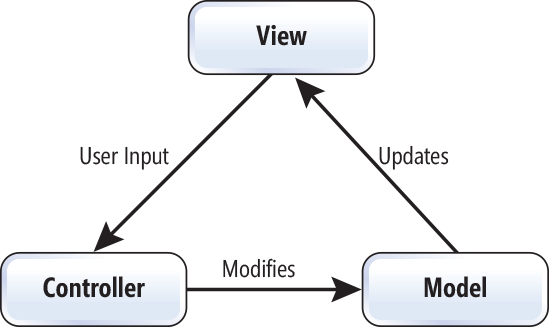
\includegraphics[scale=0.5]{img/mvc}  
			\caption{Struttura del pattern MVC}
		\end{figure}
		
		\begin{itemize}	
			\item \textbf{Descrizione} \\ Model View Controller è un design pattern architetturale che permette di dividere l'architettura del sistema che si intende sviluppare in tre blocchi:
			\begin{itemize}
				\item \textbf{il modello} che contiene le classi con i metodi di accesso ai dati;
				\item \textbf{la vista} che contiene le classi che permettono all'utente di visualizzare i dati e di interagire con il modello;
				\item \textbf{il controllore} che si occupa di fare da tramite tra vista e modello, ovvero riceve i comandi dell'utente attraverso la vista e va a cambiare lo stato del modello di conseguenza, successivamente aggiorna la vista.				
			\end{itemize}
			
			\item \textbf{Vantaggi} \\
			Questo pattern architetturale permette il riuso del codice in quanto molte parti di lavoro sono indipendenti. Ad esempio il modello creato potrà essere utilizzato con diverse viste. \\ Grazie all'indipendenza di alcune parti è semplice dividere il lavoro tra più componenti di un team e sarà quindi più facile anche la manutenzione.
			\utilizzo \\
			Nel nostro progetto il pattern MVC è usato nella parte client dell'architettura. 
		\end{itemize}
		
		\newpage
		
\subsection{Pattern creazionali}
	\subsubsection{Abstract Factory}
	
	\begin{figure}[!h]
		\centering
		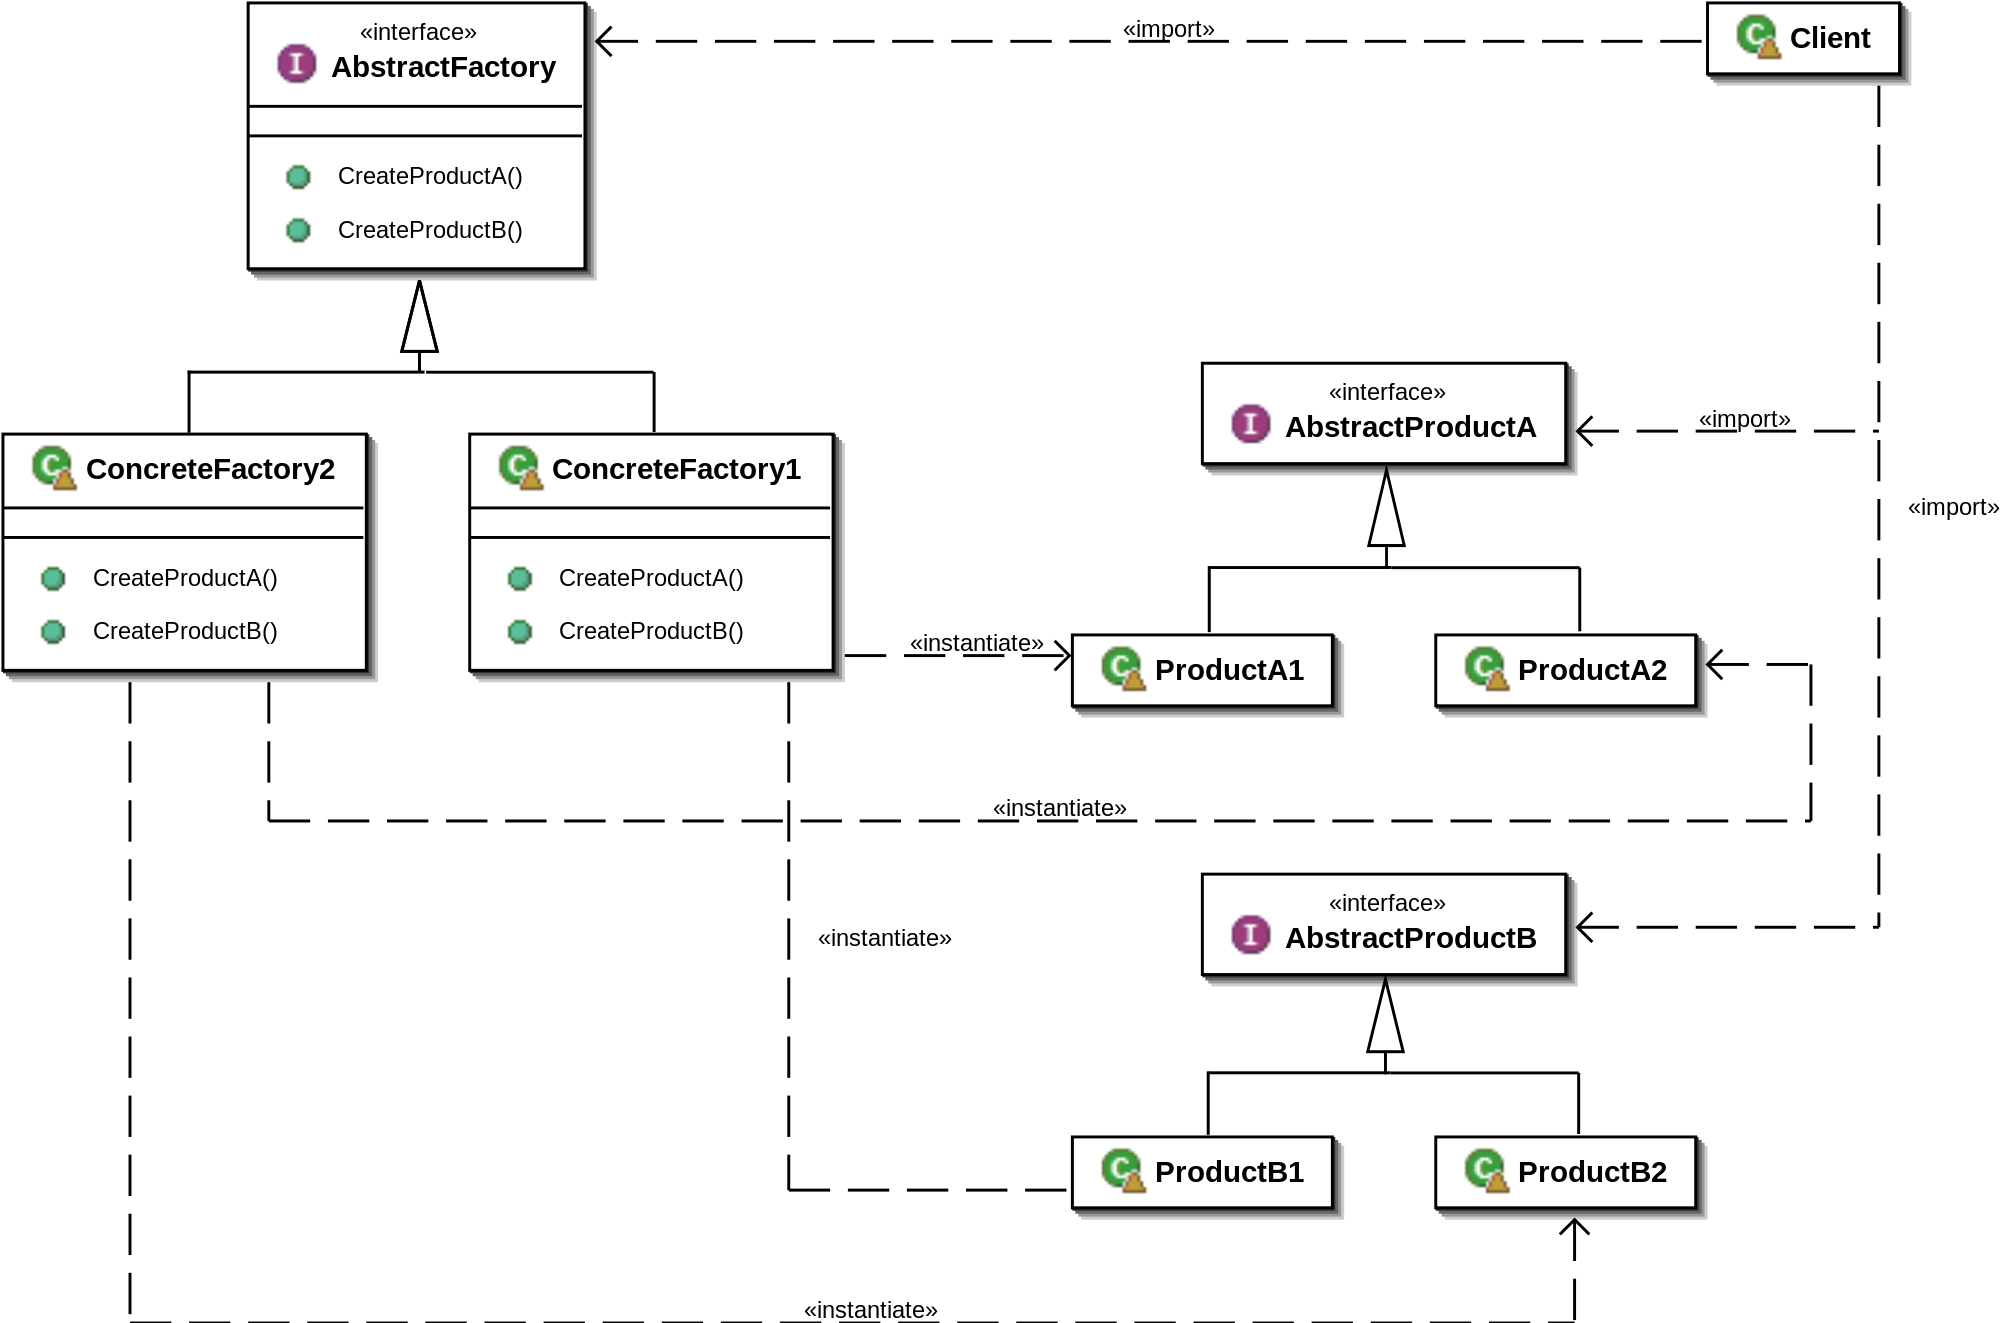
\includegraphics[scale=0.2]{img/abstract_factory}  
		\caption{Struttura del pattern Abstract Factory}
	\end{figure}
	
		\begin{itemize}
			\item \textbf{Descrizione}\\ 
			Il design pattern Abstract Factory fornisce un'interfaccia per creare famiglie di prodotti senza specificare classi concrete. Ogni famiglia di prodotti ha una classe base astratta da cui derivano delle classi concrete. Queste classi concrete sono istanziate dalle classi concrete della factory corrispondenti.
			% immagine di esempio
			
			\item \textbf{Vantaggi}\\ 
			Questo design pattern offre vantaggi quando si vogliono modellare famiglie di prodotti che potranno essere ampliate nel futuro. Le modifiche necessarie ad aggiungere nuovi elementi alle famiglie saranno essenzialmente due, aggiungere una classe in ogni famiglia di prodotti ed un solo metodo nella factory.
			\utilizzo \\ 
			Nel nostro progetto abbiamo utilizzato questo design pattern per modellare i tipi di quiz che vengono proposti agli utenti. Abbiamo infatti deciso di utilizzare solo due famiglie di quiz, quindi vi è la necessità di avere modo in futuro di ampliare le tipologie di quiz disponibili in modo semplice ed efficace.
			
			\begin{figure}[!h]
				\centering
				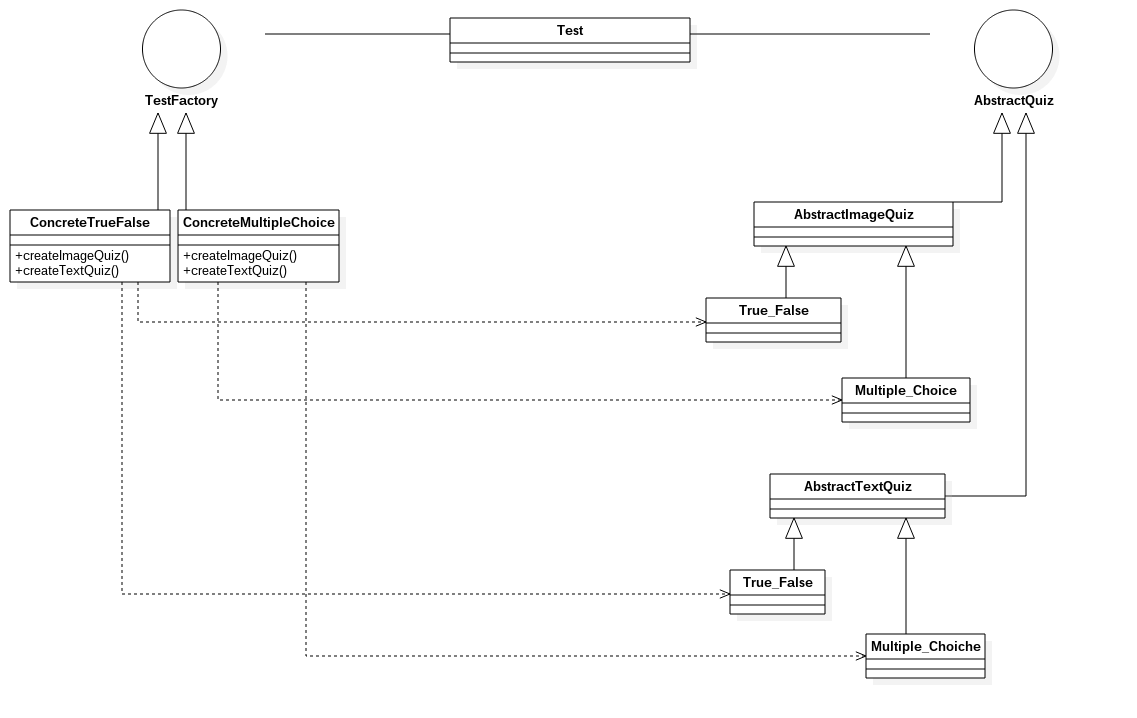
\includegraphics[scale=0.4]{img/our_abstract_factory}  
				\caption{Utilizzo di Abstract Factory nel progetto}
			\end{figure}
			
		\end{itemize}
	 \newpage
	 
	\subsubsection{Singleton}
		\begin{figure}[!h]
			\centering
			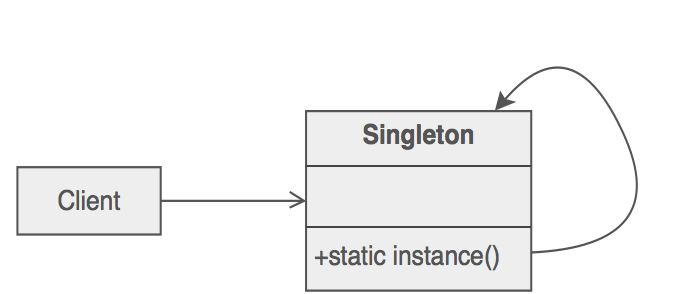
\includegraphics[scale=0.4]{img/singleton}  
			\caption{Struttura del pattern Singleton}
		\end{figure}
		
		\begin{itemize}
			\item \textbf{Descrizione}\\ 
			 Assicura l'esistenza di un'unica istanza di una classe e permette di avere un punto di accesso globale a questa.
			 Per rendere possibile ciò si mette il costruttore protetto o privato e si crea un metodo statico, chiamato factory, che fornisce l’accesso all'unica copia dell’oggetto (contiene un puntatore all’unica istanza).			 
			 \item \textbf{Vantaggi}\\ 
			 Se, al contrario di quanto avviene utilizzando Singleton, venisse reso visibile il costruttore della classe non si potrebbe garantire che esista un solo esemplare della classe. Un altro modo di procedere potrebbe essere quello di dichiarare una variabile globale, ma in questo modo si ``ruberebbe'' un nome al namespace globale.
			 Sigleton permette inoltre di dichiarare sottoclassi.			 
			 \utilizzo \\ 
			 Nel nostro progetto abbiamo creato un singleton per ``LoginManager'' che contiene i dati relativi a i dati di login dell'utente che sta utilizzando l'applicazione.
			 
			 	\begin{figure}[!h]
			 		\centering
			 		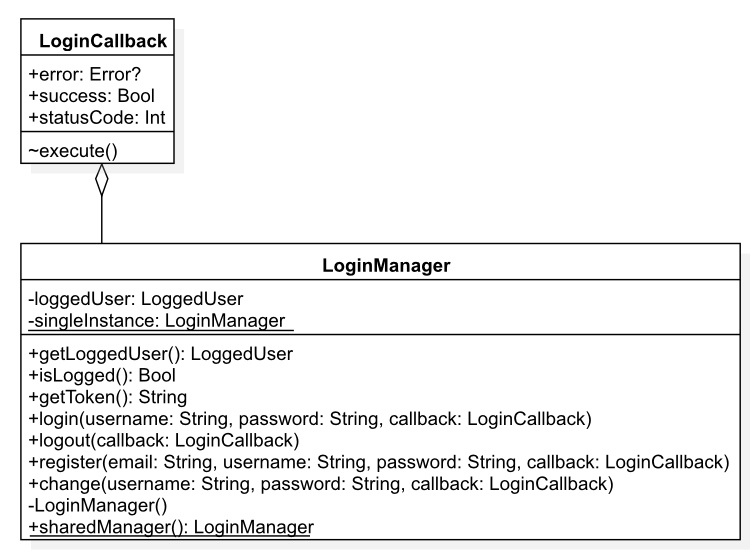
\includegraphics[scale=0.4]{img/package/png/client--loginmanager}  
			 		\caption{Utilizzo di Abstract Factory nel progetto}
			 	\end{figure}
			 
		\end{itemize}
		
		
		


\end{document}
